% A LaTeX template for ARTICLE version of the MSc Thesis submissions to 
% Politecnico di Milano (PoliMi) - School of Industrial and Information Engineering
%
% S. Bonetti, A. Gruttadauria, G. Mescolini, A. Zingaro
% e-mail: template-tesi-ingind@polimi.it
%
% Last Revision: October 2021
%
% Copyright 2021 Politecnico di Milano, Italy. Inc. NC-BY

\documentclass[11pt,a4paper]{article} 

%------------------------------------------------------------------------------
%\tREQUIRED PACKAGES AND  CONFIGURATIONS
%------------------------------------------------------------------------------
% PACKAGES FOR TITLES
\usepackage{titlesec}
\usepackage{color}

% PACKAGES FOR LANGUAGE AND FONT
\usepackage[utf8]{inputenc}
\usepackage[english]{babel}
\usepackage[T1]{fontenc} % Font encoding

% PACKAGES FOR IMAGES
\usepackage{graphicx}
\graphicspath{{Images/}}
\usepackage{eso-pic} % For the background picture on the title page
\usepackage{subfig} % Numbered and caption subfigures using \subfloat
\usepackage{caption} % Coloured captions
\usepackage{transparent}

% STANDARD MATH PACKAGES
\usepackage{amsmath}
\usepackage{amsthm}
\usepackage{bm}
\usepackage[overload]{empheq}  % For braced-style systems of equations

% PACKAGES FOR TABLES
\usepackage{tabularx}
\usepackage{longtable} % tables that can span several pages
\usepackage{colortbl}

% PACKAGES FOR ALGORITHMS (PSEUDO-CODE)
\usepackage{algorithm}
\usepackage{algorithmic}

% PACKAGES FOR REFERENCES & BIBLIOGRAPHY
\usepackage[colorlinks=true,linkcolor=black,anchorcolor=black,citecolor=black,filecolor=black,menucolor=black,runcolor=black,urlcolor=black]{hyperref} % Adds clickable links at references
\usepackage{cleveref}
\usepackage[square, numbers, sort&compress]{natbib} % Square brackets, citations sorted by appearance in the text and compressed
\bibliographystyle{unsrtnat} % You may use a different style adapted to your field

% PACKAGES FOR THE APPENDIX
\usepackage{appendix}

% PACKAGES FOR ITEMIZE & ENUMERATES 
\usepackage{enumitem}

% OTHER PACKAGES
\usepackage{thmtools,xcolor} % Coloured "Theorem"
\usepackage{comment} % Comment part of code
\usepackage{fancyhdr} % Fancy headers and footers
\usepackage{lipsum} % Insert dummy text
\usepackage{tcolorbox} % Create coloured boxes (e.g. the one for the key-words)

%-------------------------------------------------------------------------
%\tNEW COMMANDS DEFINED
%-------------------------------------------------------------------------
% EXAMPLES OF NEW COMMANDS -> here you see how to define new commands
\newcommand{\bea}{\begin{eqnarray}} % Shortcut for equation arrays
\newcommand{\eea}{\end{eqnarray}}
\newcommand{\e}[1]{\times 10^{#1}}  % Powers of 10 notation
\newcommand{\mathbbm}[1]{\text{\usefont{U}{bbm}{m}{n}#1}} % From mathbbm.sty
\newcommand{\pdev}[2]{\frac{\partial#1}{\partial#2}}
% NB: you can also override some existing commands with the keyword \renewcommand

%----------------------------------------------------------------------------
%\tADD YOUR PACKAGES (be careful of package interaction)
%----------------------------------------------------------------------------


%----------------------------------------------------------------------------
%\tADD YOUR DEFINITIONS AND COMMANDS (be careful of existing commands)
%----------------------------------------------------------------------------


% Do not change Configuration_files/config.tex file unless you really know what you are doing. 
% This file ends the configuration procedures (e.g. customizing commands, definition of new commands)
\input{Configuration_files/config}

% Insert here the info that will be displayed into your Title page 
% -> title of your work
\renewcommand{\title}{Pneumonia Detection Using Anchor-Free Object Detection}
% -> author name and surname
\renewcommand{\author}{Francesco Rausa}
% -> MSc course
\newcommand{\course}{Numerical Analysis for Machine Learning}
% -> advisor name and surname
%\newcommand{\advisor}{Prof. Name Surname}
% IF AND ONLY IF you need to modify the co-supervisors you also have to modify the file Configuration_files/title_page.tex (ONLY where it is marked)
%\newcommand{\firstcoadvisor}{Name Surname} % insert if any otherwise comment
%\newcommand{\secondcoadvisor}{Name Surname} % insert if any otherwise comment
% -> author ID
\newcommand{\ID}{10833982}
% -> academic year
\newcommand{\YEAR}{2025-2026}
% -> abstract (only in English)
\renewcommand{\abstract}{
This project aims to re-implement and investigate an anchor-free object detection framework for pneumonia localization in chest X-ray images. The work is motivated by the framework proposed for pneumonia detection on the RSNA dataset, while adopting FCOS as the main reference for the design of the detector. The resulting architecture combines a ResNet backbone with a Feature Pyramid Network (FPN) and detection heads for classification, bounding-box regression, and centerness prediction. The implementation is evaluated using both ImageNet- and Chest-Xray-pretrained backbones and considers different ResNet depths. Particular attention is given to training stability, leading to the adoption of training strategies including learning-rate scheduling, backbone freezing and gradual unfreezing, gradient clipping, and exponential moving average (EMA) of the model parameters. The final system therefore preserves the medical application and dataset setting of the reference pneumonia study while following the anchor-free, fully convolutional formulation of FCOS, with additional implementation choices introduced to improve robustness and flexibility in the target application.
}

% -> key-words (only in English)
\newcommand{\keywords}{anchor-free object detection, FCOS, pneumonia detection, chest X-ray, ResNet, transfer learning}

%-------------------------------------------------------------------------
%\tBEGIN OF YOUR DOCUMENT
%-------------------------------------------------------------------------
\begin{document}

%-----------------------------------------------------------------------------
% TITLE PAGE
%-----------------------------------------------------------------------------
% Do not change Configuration_files/TitlePage.tex (Modify it IF AND ONLY IF you need to add or delete the Co-advisors)
% This file creates the Title Page of the document
\input{Configuration_files/title_page}

%%%%%%%%%%%%%%%%%%%%%%%%%%%%%%
%%     THESIS MAIN TEXT     %%
%%%%%%%%%%%%%%%%%%%%%%%%%%%%%%

%-----------------------------------------------------------------------------
% TITLE PAGE
%-----------------------------------------------------------------------------
% Do not change Configuration_files/TitlePage.tex (Modify it IF AND ONLY IF you need to add or delete the Co-advisors)
% This file creates the Title Page of the document
%\input{Configuration_files/title_page}

%%%%%%%%%%%%%%%%%%%%%%%%%%%%%%
%%     THESIS MAIN TEXT     %%
%%%%%%%%%%%%%%%%%%%%%%%%%%%%%%

%-----------------------------------------------------------------------------
% INTRODUCTION
%-----------------------------------------------------------------------------

\section{Introduction}
\label{sec:introduction}

Pneumonia is a major respiratory disease and remains an important cause of morbidity and mortality worldwide. 
Chest X-ray imaging is one of the most widely used tools for its assessment, but the interpretation of radiographs is challenging because the manifestations of pneumonia can be subtle, heterogeneous, and spatially overlapping with other abnormalities. 
In addition to determining whether pneumonia is present, identifying its precise location is particularly relevant for computer-assisted analysis, as the affected regions may vary substantially in size, shape, and appearance. 
The availability of the RSNA Pneumonia Detection Challenge dataset has made it possible to investigate deep learning methods for the automated localization of pneumonia in chest radiographs. 
In particular, Wu et al.~\cite{wu2024pneumonia} proposed an anchor-free object detection framework for this task, demonstrating the potential of fully convolutional detection methods in the medical imaging domain.

Object detection traditionally relies on predefined anchor boxes, whose dimensions, aspect ratios, and scales must be selected before training. 
These design choices introduce additional hyperparameters and can be particularly restrictive when the target objects exhibit large variations in size and shape. 
Anchor-free detectors address this issue by removing the need for predefined boxes and directly predicting object information from spatial locations in the feature maps. 
Among these approaches, Fully Convolutional One-Stage Object Detection (FCOS) formulates detection as a dense, per-location prediction problem, in which each spatial location is associated with a bounding-box regression and a classification prediction, together with a centerness score used to suppress low-quality detections~\cite{tian2019fcos}. 
This formulation is especially interesting in the context of pneumonia localization, where the shape and extent of the detected regions may vary considerably.

The objective of this project is to re-implement the pneumonia detection framework proposed by Wu et al.~\cite{wu2024pneumonia}, with a particular focus on the FCOS detection paradigm. 
Rather than reproducing the reference implementation in every detail, the project develops an FCOS-based detector and investigates the effect of different backbone configurations. 
The detector is built upon a ResNet backbone~\cite{he2016resnet} and a Feature Pyramid Network (FPN)~\cite{lin2017fpn}, which provides feature representations at multiple spatial scales. 
The resulting feature maps are processed by FCOS-style detection heads that predict classification, bounding-box regression, and centerness at each pyramid level. 
Focal Loss~\cite{lin2017focal} is employed to address the severe foreground-background imbalance arising from dense prediction.

A further objective of the project is to investigate how the initialization and depth of the backbone affect the resulting detector. 
Four backbone configurations are considered: ResNet-50 and ResNet-101 initialized with ImageNet-pretrained weights, and ResNet-50 and ResNet-101 initialized through a preliminary Chest-Xray classification pretraining stage. 
In the latter case, the ResNet is first trained to distinguish normal from pneumonia chest radiographs and is subsequently reused as the feature extractor of the detection network. 
This allows the study to distinguish the effect of increasing network depth from that of adapting the learned representation to the target medical domain.

The implementation also investigates training strategies aimed at improving optimization stability. 
In particular, the training procedure includes learning-rate scheduling, temporary backbone freezing followed by gradual unfreezing, gradient clipping, and an exponential moving average of the trainable parameters. 
These choices are motivated by the optimization difficulties observed during the development of the detector and are intended to provide a more stable training procedure while preserving the FCOS formulation as the main detection reference.

The main objectives of this project can therefore be summarized as follows:

\begin{itemize}
    \item re-implement an anchor-free pneumonia detection system based on the RSNA dataset and the FCOS formulation;
    \item investigate the role of the backbone architecture by comparing ResNet-50 and ResNet-101;
    \item compare generic ImageNet pretraining with domain-specific Chest-Xray pretraining;
    \item analyze the effects of different training strategies adopted to improve optimization stability.
\end{itemize}





%-----------------------------------------------------------------------------
% DATASET
%-----------------------------------------------------------------------------



\section{Dataset}
\label{sec:dataset}

Two different datasets are used in this project for two distinct stages of the
pipeline. The Chest-Xray dataset is employed during the preliminary
classification pretraining of the ResNet backbone, whereas the RSNA Pneumonia
Detection dataset is used for training and evaluating the final object
detector.

\subsection{Chest-Xray Classification Dataset}
\label{subsec:chest_xray_dataset}

The first dataset is used to pretrain the ResNet backbone on a binary
classification task. The dataset is organized into three independent splits:
\texttt{train}, \texttt{val}, and \texttt{test}. Each split contains two
class directories, \texttt{NORMAL} and \texttt{PNEUMONIA}, as illustrated by
the following structure:

\begin{verbatim}
data/chest_xray/
|-- train/
|   |-- NORMAL/
|   `-- PNEUMONIA/
|-- val/
|   |-- NORMAL/
|   `-- PNEUMONIA/
`-- test/
    |-- NORMAL/
    `-- PNEUMONIA/
\end{verbatim}

The dataset contains 5,856 chest X-ray images in total. The training,
validation, and test sets contain 4,684, 585, and 587 images, respectively.
The class distribution is highly consistent across the three splits, with
approximately 73\% of the images belonging to the PNEUMONIA class and 27\%
to the NORMAL class.

\begin{table}[H]
    \centering
    \caption{Chest-Xray class distribution.}
    \label{table:classification_dataset}
    \begin{tabular}{lrrrr}
        \hline
        \textbf{Split} &
        \textbf{NORMAL} &
        \textbf{PNEUMONIA} &
        \textbf{Total} &
        \textbf{PNEUMONIA (\%)} \\
        \hline
        Train & 1266 & 3418 & 4684 & 72.97 \\
        Validation & 158 & 427 & 585 & 72.99 \\
        Test & 159 & 428 & 587 & 72.91 \\
        \hline
        \textbf{Total} & \textbf{1583} &
        \textbf{4273} & \textbf{5856} & \textbf{72.97} \\
        \hline
    \end{tabular}
\end{table}

The dataset is therefore imbalanced towards the PNEUMONIA class, with
approximately 2.7 pneumonia images for every normal image.

\begin{figure}[H]
    \centering
    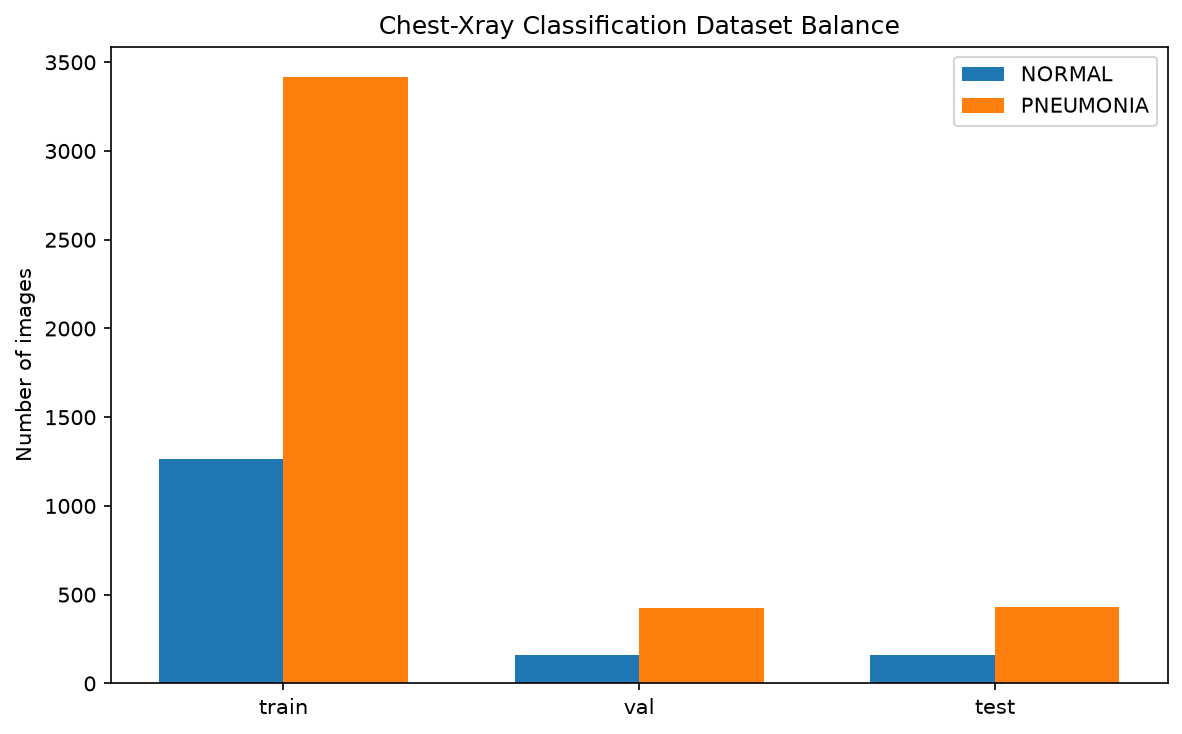
\includegraphics[
        width=0.6\textwidth
    ]{Images/dataset_analysis/chest_xray_class_balance.png}
    \caption{Chest-Xray class distribution across the three splits.}
    \label{fig:chest_xray_balance}
\end{figure}


\subsection{RSNA Pneumonia Detection Dataset}
\label{subsec:rsna_dataset}

The second dataset is the RSNA Pneumonia Detection Challenge dataset, which
is used for the object detection task. It contains chest radiographs stored
as DICOM files together with a separate CSV file containing the corresponding
pneumonia annotations.

The dataset is organized as follows:

\begin{verbatim}
data/rsna-pneumonia-detection-challenge/
|-- stage_2_train_images/
|   |-- <patientId>.dcm
|   |-- <patientId>.dcm
|   `-- ...
`-- stage_2_train_labels.csv
\end{verbatim}

A total of 26,684 DICOM images are present in the dataset. According to the
annotation file, 6,012 images contain at least one positive pneumonia
annotation, while 20,672 images do not contain a positive pneumonia
annotation. This corresponds to approximately 22.53\% positive images and
77.47\% negative images.

\begin{table}[H]
    \centering
    \caption{RSNA image-level class distribution.}
    \label{table:rsna_dataset}
    \begin{tabular}{lrr}
        \hline
        \textbf{Category} &
        \textbf{Number of images} &
        \textbf{Percentage} \\
        \hline
        Positive & 6012 & 22.53\% \\
        Negative & 20672 & 77.47\% \\
        \hline
        \textbf{Total} & \textbf{26684} & \textbf{100.00\%} \\
        \hline
    \end{tabular}
\end{table}

The RSNA dataset is therefore strongly imbalanced at the image level, with
most images containing no positive pneumonia annotation. This distribution
should be distinguished from the foreground-background imbalance introduced
by dense object detection, which is discussed separately in
Section~\ref{sec:losses}.

\begin{figure}[H]
    \centering
    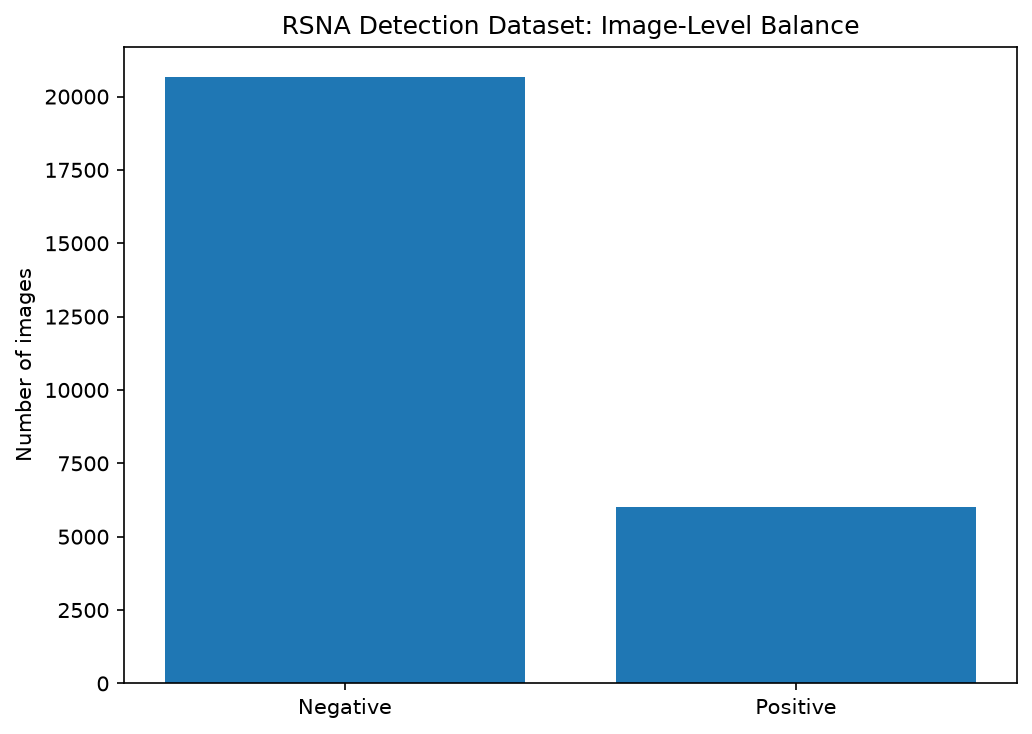
\includegraphics[
        width=0.60\textwidth
    ]{Images/dataset_analysis/rsna_image_balance.png}
    \caption{Positive and negative RSNA images.}
    \label{fig:rsna_image_balance}
\end{figure}




% -----------------------------------------------------------------------------
% BOUNDING-BOX STATISTICS
% -----------------------------------------------------------------------------



\section{Network Architecture}
\label{sec:architecture}

The proposed detector is composed of three main components: a ResNet backbone,
a Feature Pyramid Network (FPN), and a set of detection heads. The overall
architecture follows the fully convolutional and anchor-free formulation of
FCOS~\cite{tian2019fcos}, while the individual components are implemented and
adapted to the pneumonia detection task.

\subsection{ResNet Backbone}
\label{subsec:resnet_backbone}

The first component of the network is a Residual Network (ResNet), introduced
by He et al.~\cite{he2016resnet}. The main motivation behind ResNet is the
difficulty of optimizing very deep neural networks. In particular, the
original work identified a degradation problem in which increasing the depth
of a conventional ``plain'' network could lead to higher training error
rather than improved performance. The authors showed that this behaviour was
not simply caused by overfitting, and that the problem could persist even in
the presence of Batch Normalization and apparently well-behaved gradient
norms. They therefore interpreted the phenomenon primarily as an optimization
difficulty associated with very deep networks.

The key idea introduced by ResNet is residual learning. Instead of directly
learning a desired mapping $H(x)$, a stack of layers is trained to learn the
residual function

\begin{equation}
F(x) = H(x) - x,
\end{equation}

so that the original mapping can be written as

\begin{equation}
H(x) = F(x) + x.
\end{equation}

This formulation is implemented through a shortcut connection that directly
forwards the input to the output of the residual branch. According to the
authors, this reformulation makes the optimization easier, particularly when
the desired transformation is close to an identity mapping. In such cases,
the residual branch can approach zero rather than requiring a stack of
non-linear layers to explicitly learn an identity transformation
~\cite{he2016resnet}.

\subsubsection{Bottleneck Residual Block}
\label{subsubsec:bottleneck}

The ResNet-50 and ResNet-101 models used in this project employ the
bottleneck residual block introduced in the original ResNet architecture.
Unlike the basic two-layer residual block, the bottleneck block consists of
three convolutions:

\begin{enumerate}
    \item a $1\times1$ convolution that projects the input into a lower
    dimensional feature space;
    \item a $3\times3$ convolution that performs the main spatial feature
    extraction;
    \item a final $1\times1$ convolution that restores the expanded channel
    dimension.
\end{enumerate}

For an input with $C$ channels, the bottleneck representation uses an
intermediate dimensionality of $C/4$ in the conceptual bottleneck view, while
the final convolution expands the representation by a factor of four. In the
implementation used in this project, this expansion is explicitly defined
as

\begin{equation}
C_{\mathrm{out}} = 4C_{\mathrm{bottleneck}}.
\end{equation}

The three convolutions are combined with Batch Normalization and ReLU
activations, while the original input is propagated through a shortcut branch.
The residual output is therefore computed as

\begin{equation}
y = \mathrm{ReLU}\left(F(x) + S(x)\right),
\end{equation}

where $F(x)$ denotes the three-layer residual branch and $S(x)$ denotes the
shortcut. When the input and output dimensions are compatible, $S(x)$ is an
identity mapping. When their dimensions differ, a projection shortcut based
on a $1\times1$ convolution and Batch Normalization is used to match the
dimensions~\cite{he2016resnet}.

\subsubsection{ResNet-50 and ResNet-101 Structure}
\label{subsubsec:resnet_structure}

The main difference between ResNet-50 and ResNet-101 is the number of
bottleneck blocks stacked at each stage. Following the architecture reported
by He et al.~\cite{he2016resnet}, the four residual stages are organized as

\begin{equation}
\mathrm{ResNet\mbox{-}50} = [3,4,6,3]
\end{equation}

and

\begin{equation}
\mathrm{ResNet\mbox{-}101} = [3,4,23,3].
\end{equation}

\begin{figure}[H]
    \centering
    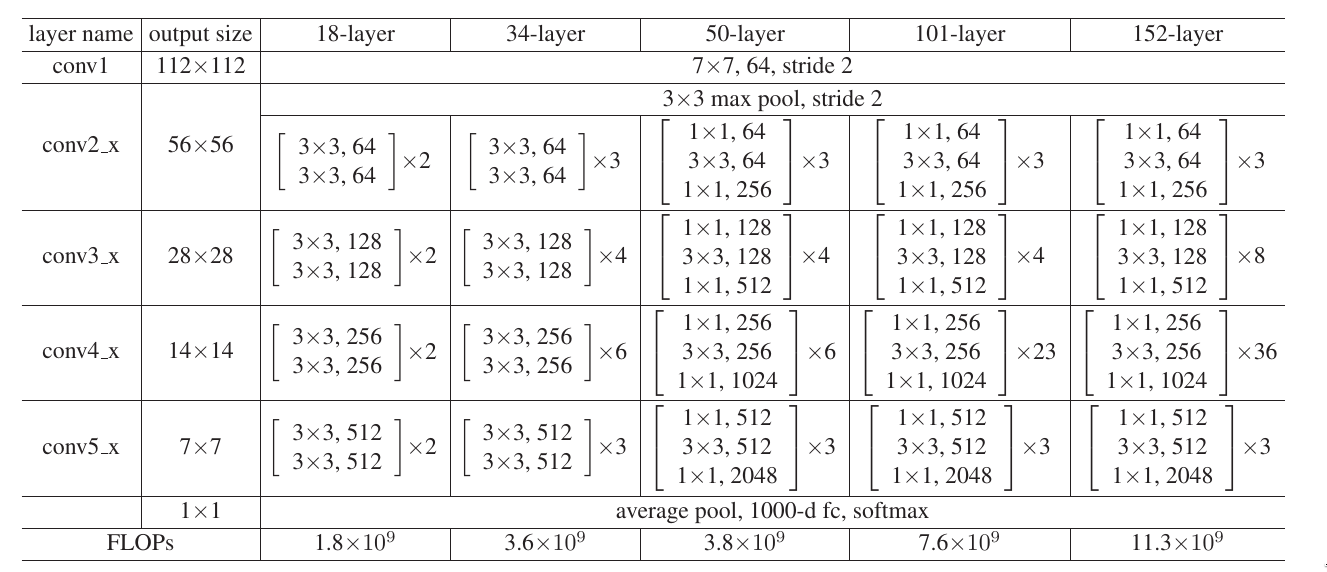
\includegraphics[
        width=0.75\textwidth
    ]{Images/arch/resnet_struct_general.png}
    \caption{ResNet-50 and ResNet-101 stage structure.}
    \label{fig:resnet_structure}
\end{figure}


The number of blocks is therefore increased almost entirely in the third
residual stage. The resulting feature representations have the following
channel dimensions:

\begin{center}
\begin{tabular}{lccc}
    \hline
    \textbf{Stage} & \textbf{Feature} & \textbf{Channels} &
    \textbf{ResNet-50 / 101 blocks} \\
    \hline
    Initial & -- & 64 & -- \\
    $conv2_x$ & $C_2$ & 256 & 3 / 3 \\
    $conv3_x$ & $C_3$ & 512 & 4 / 4 \\
    $conv4_x$ & $C_4$ & 1024 & 6 / 23 \\
    $conv5_x$ & $C_5$ & 2048 & 3 / 3 \\
    \hline
\end{tabular}
\end{center}

The spatial resolution is progressively reduced throughout the network,
while the number of feature channels increases. This hierarchical structure
is particularly suitable for detection because it provides feature
representations at different levels of abstraction.

The original ResNet paper reports the same bottleneck configurations for
ResNet-50 and ResNet-101, with the corresponding difference in depth and
computational cost~\cite{he2016resnet}.

\subsubsection{Implementation}
\label{subsubsec:resnet_implementation}

Two implementations of the ResNet backbone were used during the development
and evaluation of the detection pipeline. The first relies on the standard
implementations provided by \texttt{torchvision}, which were used to obtain
the established ResNet-50 and ResNet-101 architectures and, in particular,
their ImageNet-pretrained weights. In parallel, a custom PyTorch
implementation of ResNet was developed to provide direct control over the
residual blocks, intermediate stage outputs, and parameter loading. This
custom implementation was useful for inspecting and validating the internal
operations of the backbone, testing different configurations, and integrating
the selected feature maps directly with the Feature Pyramid Network (FPN).

The custom implementation follows the standard ResNet architecture, and the
same implementation is used for both depths; only the number of bottleneck
blocks differs between ResNet-50 and ResNet-101. The use of both the
\texttt{torchvision} implementation and the custom implementation also
provided a way to cross-check the backbone behaviour while retaining
sufficient flexibility for subsequent experiments and modifications to the
detection pipeline.

\subsection{Feature Pyramid Network}
\label{subsec:fpn}

The second component of the detector is the Feature Pyramid Network (FPN),
introduced by Lin et al.~\cite{lin2017fpn}. The main motivation behind FPN is
the need to represent objects at different spatial scales while retaining
strong semantic information at every resolution.

A convolutional backbone naturally produces a hierarchical representation of
the input image. As the network progresses towards deeper layers, repeated
downsampling reduces the spatial resolution of the feature maps, while the
features become increasingly rich in high-level semantic information.
Conversely, shallower layers preserve more accurate spatial and localization
information, but their representations are semantically weaker. The original
FPN paper refers to this discrepancy as a semantic gap between the different
levels of the feature hierarchy~\cite{lin2017fpn}.

This creates an inherent trade-off for object detection. Using only deep
features provides strong semantic representations but poor spatial
resolution, which can be particularly problematic for small objects. On the
other hand, using only shallow features preserves spatial detail but provides
less discriminative semantic information. The purpose of FPN is therefore not
simply to obtain feature maps at different scales, but to enrich the
high-resolution maps with the semantic information available in deeper
layers~\cite{lin2017fpn}.

\subsubsection{FPN Construction}
\label{subsubsec:fpn_construction}

For a ResNet backbone, the original FPN identifies the outputs of the last
residual block of each backbone stage as $C_2$, $C_3$, $C_4$, and $C_5$.
These feature maps have strides of $4$, $8$, $16$, and $32$ pixels with
respect to the input image, respectively~\cite{lin2017fpn}.

The FPN combines these feature maps through two complementary mechanisms. The
first is a top-down pathway, which propagates information from deeper,
coarser feature maps towards shallower, finer ones. The second consists of
lateral connections, which inject the spatially more precise information of
the corresponding backbone features into the top-down pathway.

The construction starts from the deepest feature map. A $1\times1$
convolution first projects $C_5$ into the feature dimension used by the
pyramid. The resulting representation is then progressively upsampled by a
factor of two and added to a lateral projection of the feature map at the
next level. A $3\times3$ convolution is finally applied to the merged feature
map in order to produce the output pyramid level.

Conceptually, the process can be expressed as

\begin{equation}
P_5 =
\mathrm{Conv}_{1\times1}(C_5),
\end{equation}

followed by

\begin{equation}
P_4 =
\mathrm{Conv}_{3\times3}
\left(
\mathrm{Conv}_{1\times1}(C_4)
+
\mathrm{Upsample}(P_5)
\right),
\end{equation}

and

\begin{equation}
P_3 =
\mathrm{Conv}_{3\times3}
\left(
\mathrm{Conv}_{1\times1}(C_3)
+
\mathrm{Upsample}(P_4)
\right).
\end{equation}

\begin{figure}[H]
    \centering
    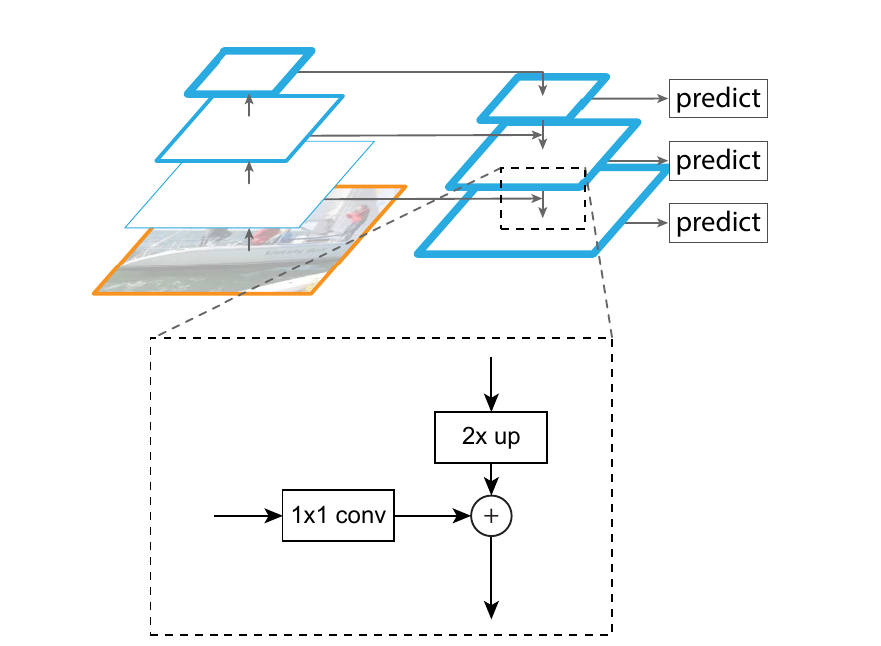
\includegraphics[width=0.42\textwidth]{Images/arch/FPN_general.png}
    \caption{Feature Pyramid Network.}
    \label{fig:fpn_general}
\end{figure}

The lateral terms preserve the spatial information of the shallower
features, while the top-down pathway transfers the stronger semantic
representation of the deeper features to higher resolutions. The resulting
feature maps therefore contain a more balanced combination of semantic
richness and spatial precision. The original FPN paper fixes the number of
channels of the pyramid features to 256 and uses the same feature dimension
at all levels~\cite{lin2017fpn}.

\subsubsection{FPN in the Implemented Detector}
\label{subsubsec:implemented_fpn}

The implementation developed in this project follows the same top-down and
lateral-connection principle, while adapting the pyramid to the requirements
of FCOS. The ResNet backbone produces four outputs,

\begin{equation}
\{C_2,C_3,C_4,C_5\},
\end{equation}

but $C_2$ is not used in the construction of the detection pyramid. The
remaining feature maps $C_3$, $C_4$, and $C_5$ are projected to 256 channels
through $1\times1$ convolutions and combined through the top-down pathway.

In the implementation, the construction therefore proceeds as follows:

\begin{equation}
C_5 \rightarrow P_5,
\end{equation}

\begin{equation}
C_4 + \mathrm{Upsample}(P_5) \rightarrow P_4,
\end{equation}

\begin{equation}
C_3 + \mathrm{Upsample}(P_4) \rightarrow P_3.
\end{equation}

The resulting three feature maps are then extended by two additional levels.
$P_6$ is generated using a $3\times3$ convolution with stride $2$ applied to
$P_5$, while $P_7$ is obtained by applying another stride-$2$ convolution to
$P_6$ after a ReLU activation.

Consequently, the final feature pyramid used by the detector is

\begin{equation}
\{P_3,P_4,P_5,P_6,P_7\},
\end{equation}

with corresponding strides

\begin{equation}
\{8,16,32,64,128\}.
\end{equation}

This five-level configuration is particularly suitable for FCOS because
different object sizes can be handled at different levels of the pyramid.
The finer levels provide a denser spatial representation, whereas the
coarser levels provide a larger receptive field and are therefore more
appropriate for larger objects.

\subsubsection{Relation to FPN and FCOS}
\label{subsubsec:fpn_comparison}

The implemented pyramid follows FCOS rather than reproducing the feature
construction of Wu et al.~\cite{wu2024pneumonia}. The reference framework
uses five backbone outputs, projected independently to feature levels with
strides $8,16,32,64,128$, whereas the present detector builds $P_3$--$P_5$
through the top-down FPN pathway and derives $P_6$ and $P_7$ with stride-2
convolutions. Thus, the number and strides of the levels are shared, but the
feature fusion is different. This is the main architectural choice that
makes the implementation closer to FCOS than to a literal re-implementation
of the reference pneumonia detector~\cite{tian2019fcos}.
\begin{figure}[H]
    \centering
    \subfloat[FCOS\label{fig:fcos_fpn}]{%
        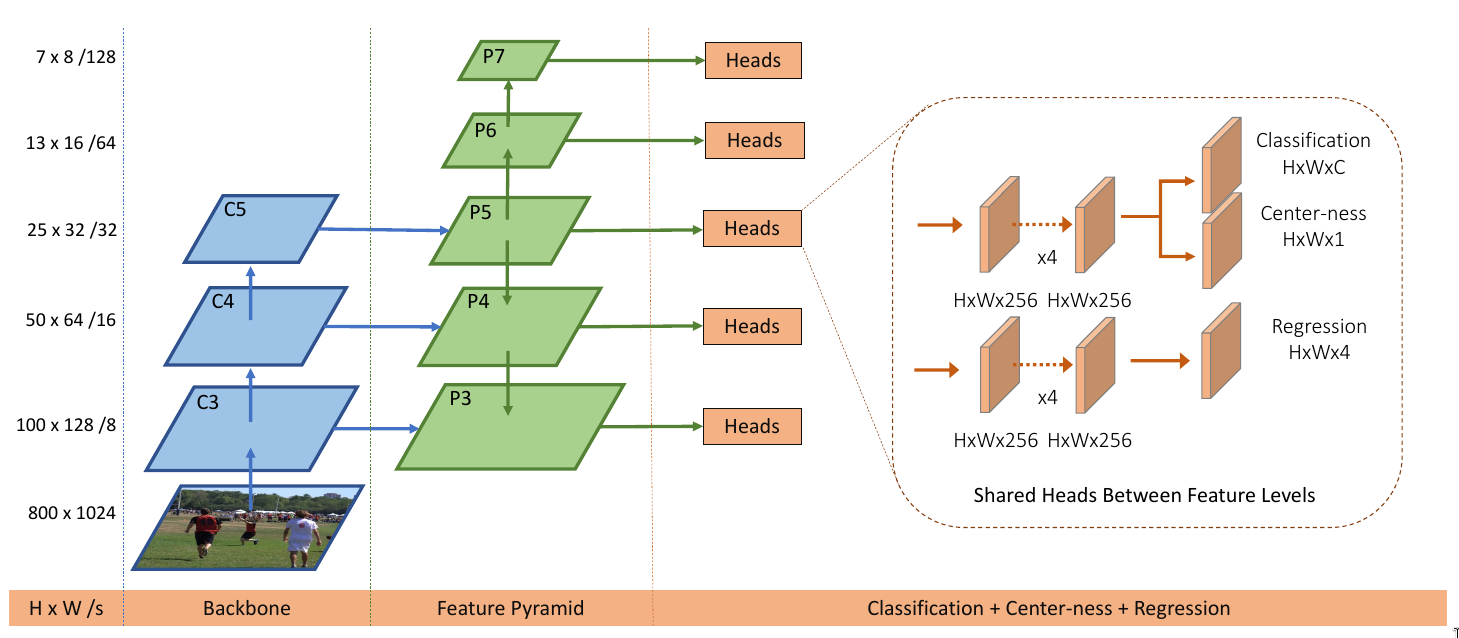
\includegraphics[width=0.42\textwidth]{Images/arch/FCOS_FPN.png}%
    }
    \hspace{0.06\textwidth}
    \subfloat[Reference pneumonia framework\label{fig:pneumonia_fpn}]{%
        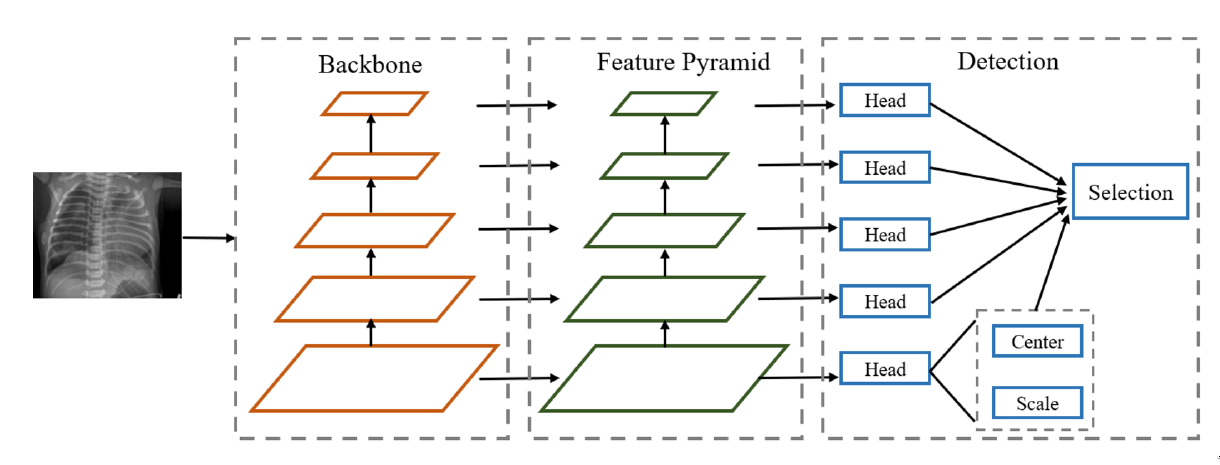
\includegraphics[width=0.42\textwidth]{Images/arch/Pneumonia_FPN.png}%
    }
    \caption{FCOS and reference pneumonia feature pyramids.}
    \label{fig:fpn_comparison}
\end{figure}
\subsubsection{Architectural Choice}
\label{subsubsec:architectural_choice}

The choice to follow FCOS rather than reproduce the reference pneumonia
architecture exactly is central to the project. The original FPN builds a
top-down hierarchy by combining deeper semantic features with lateral
connections from shallower layers~\cite{lin2017fpn}. FCOS uses this principle
with $P_3$--$P_5$ obtained from $C_3$--$C_5$ and extends the pyramid with
$P_6$ and $P_7$ through stride-2 convolutions~\cite{tian2019fcos}. This is the
same feature-level structure used here.

The reference pneumonia framework also operates on five levels with strides
$8,16,32,64,128$, but constructs the levels from five backbone outputs that
are projected independently~\cite{wu2024pneumonia}. Thus the two approaches
share the multi-scale idea and the same nominal stride progression, but not
the internal feature fusion. For this project, the FCOS construction was
preferred because the goal was to study the anchor-free detector itself and
not simply reproduce the reference implementation as a black box.

This distinction is important when interpreting the experiments: the results
evaluate a specific FCOS-style detector applied to the RSNA pneumonia task,
rather than a strict reproduction of every architectural and optimization
choice made by Wu et al.~\cite{wu2024pneumonia}.

\subsection{Detection Head}
\label{subsec:detection_head}

The detection head converts the feature maps produced by the FPN into the
quantities required by an anchor-free detector. Since no anchor boxes are
used, the predictions are associated directly with spatial locations on each
pyramid level. The implemented head follows the FCOS decomposition into
classification, bounding-box regression and centerness, while keeping a
simpler internal structure.

For each of the five levels $P_3$--$P_7$, a separate \texttt{DetectionHead}
module is instantiated. Each input feature map has 256 channels. The head
contains two feature towers. The classification tower applies a $3\times3$
convolution, Group Normalization and ReLU, followed by a $1\times1$
convolution that produces one classification logit per location. The second
tower has the same $3\times3$--GroupNorm--ReLU structure and is used jointly
by the regression and centerness branches. Two $1\times1$ convolutions then
produce the four LTRB regression values and one centerness value.

For a pyramid level $P_i$, the classification features can be written as

\begin{equation}
F_{\mathrm{cls}}=
\mathrm{ReLU}\left(\mathrm{GN}\left(\mathrm{Conv}_{3\times3}(P_i)\right)\right),
\end{equation}

with classification output

\begin{equation}
C_i=\mathrm{Conv}_{1\times1}^{\mathrm{cls}}(F_{\mathrm{cls}}).
\end{equation}

The regression tower is computed independently as

\begin{equation}
F_{\mathrm{reg}}=
\mathrm{ReLU}\left(\mathrm{GN}\left(\mathrm{Conv}_{3\times3}(P_i)\right)\right),
\end{equation}

from which

\begin{equation}
R_i=\mathrm{Conv}_{1\times1}^{\mathrm{reg}}(F_{\mathrm{reg}}),
\qquad
S_i=\mathrm{Conv}_{1\times1}^{\mathrm{ctr}}(F_{\mathrm{reg}})
\end{equation}

are obtained. Here $C_i$, $R_i$ and $S_i$ denote classification,
regression and centerness predictions, respectively.

This structure is close to FCOS at the functional level, since classification
and localization are explicitly separated and centerness is predicted from
the regression features~\cite{tian2019fcos}. There are, however, two relevant
differences. First, the present implementation uses the same regression
feature representation for both LTRB regression and centerness. Second, the
head parameters are not shared across pyramid levels: five independent
\texttt{DetectionHead} modules are used. These are implementation choices
rather than architectural claims about the original FCOS model.

The reference pneumonia detector also uses five feature levels, but its head
is organized as a classification/localization module with a different scale
selection mechanism~\cite{wu2024pneumonia}. The present implementation keeps
the FCOS-style target assignment and centerness formulation instead. This
makes the distinction between the project and a literal re-implementation of
the reference model explicit.

The final output is therefore one classification value, four regression
values and one centerness value at each spatial location of every FPN level.
Although the current task is binary pneumonia detection, this separation
would also allow the classification branch to be extended to multiple lesion
classes without changing the localization representation.

\section{Target Assignment}
\label{sec:target_assignment}

In an anchor-free detector, the network does not regress bounding boxes
relative to predefined anchors. Instead, predictions are generated at the
spatial locations of each FPN feature map. The target generation stage is
therefore responsible for determining which locations correspond to
ground-truth objects and for converting the associated bounding boxes into
the representation expected by the detection heads.

For each FPN level, the target generator receives the ground-truth bounding
boxes, the spatial dimensions of the corresponding feature map, and its
stride. It produces three target tensors: a binary positive mask, the four
LTRB regression distances, and a centerness target. These targets are then
used by the corresponding training losses.

\subsection{Target Generation}
\label{subsec:target_generation}

The target assignment procedure follows the main formulation of FCOS
\cite{tian2019fcos}. First, every spatial location of the feature map is
mapped back to the coordinate system of the original image. For a feature
map location $(x,y)$ and a stride $s$, the corresponding image-space
location is defined as

\begin{equation}
p_x = (x + 0.5)s,
\qquad
p_y = (y + 0.5)s.
\end{equation}

The resulting point represents the center of the receptive cell associated
with that feature-map location.

For each location, all ground-truth boxes are examined. A box can be assigned
to the location only if the location lies inside the box. If this condition
is satisfied, the four distances from the location to the box boundaries are
computed:

\begin{equation}
l = p_x - x_1,
\qquad
t = p_y - y_1,
\qquad
r = x_2 - p_x,
\qquad
b = y_2 - p_y.
\end{equation}

The tuple

\begin{equation}
(l,t,r,b)
\end{equation}

constitutes the regression target for that location.

The second assignment criterion is the regression range associated with the
FPN level. In the implemented detector, the ranges are

\begin{equation}
\begin{array}{c|c}
\textbf{FPN level} & \textbf{Regression range} \\
\hline
P_3 & [0,64) \\
P_4 & [64,128) \\
P_5 & [128,256) \\
P_6 & [256,512) \\
P_7 & [512,\infty)
\end{array}
\end{equation}

where the size of the object is determined from the maximum of the four
regression distances,

\begin{equation}
d_{\max} = \max(l,t,r,b).
\end{equation}

A location is therefore considered a valid positive sample only if it lies
inside the ground-truth box and $d_{\max}$ falls within the regression range
of the current FPN level. This multi-level assignment strategy follows the
principle adopted by FCOS, where different feature levels are responsible
for different object-size ranges~\cite{tian2019fcos}. The corresponding
ranges are also explicitly defined in the implementation
\cite{tian2019fcos}.

When more than one ground-truth box satisfies these conditions for the same
location, an ambiguity arises because a single location cannot simultaneously
regress multiple targets. The implemented target generator resolves this
ambiguity by selecting the matching ground-truth box with the smallest area.
This is consistent with the ambiguity-resolution rule described in FCOS
\cite{tian2019fcos}.

Once the ground-truth box has been selected, the centerness target is computed
from the four LTRB distances as

\begin{equation}
\mathrm{centerness}
=
\sqrt{
\frac{\min(l,r)}{\max(l,r)}
\cdot
\frac{\min(t,b)}{\max(t,b)}
}.
\end{equation}

The centerness value is maximized when the location lies close to the center
of the bounding box and decreases towards its boundaries. Consequently, it
provides a measure of how representative a location is for the object being
regressed.

For each feature level, the target generator therefore returns

\begin{equation}
\mathcal{T}_i =
\left\{
M_i,
L_i,
C_i
\right\},
\end{equation}

where $M_i$ is the positive-location mask, $L_i$ contains the LTRB regression
targets, and $C_i$ contains the centerness targets.





%-----------------------------------------------------------------------------
% LOSS FUNCTIONS
%-----------------------------------------------------------------------------



\section{Loss Functions}
\label{sec:losses}

The detector is trained through three complementary objectives corresponding
to the three outputs produced by each detection head: classification,
bounding-box regression, and centerness. The classification branch determines
whether a spatial location corresponds to a pneumonia instance, the
regression branch estimates the spatial extent of the corresponding
bounding box, and the centerness branch estimates the quality of the
location with respect to the center of the object.

The total training objective is defined as

\begin{equation}
\mathcal{L}
=
\lambda_{\mathrm{cls}}\mathcal{L}_{\mathrm{cls}}
+
\lambda_{\mathrm{reg}}\mathcal{L}_{\mathrm{reg}}
+
\lambda_{\mathrm{ctr}}\mathcal{L}_{\mathrm{ctr}},
\end{equation}

where $\lambda_{\mathrm{cls}}$, $\lambda_{\mathrm{reg}}$, and
$\lambda_{\mathrm{ctr}}$ weight the contribution of the three objectives.
In the present implementation, all three weights are set to one.

The overall formulation is strongly inspired by FCOS~\cite{tian2019fcos}.
In particular, the classification objective uses the Focal Loss introduced by
Lin et al.~\cite{lin2017focal}, the bounding-box regression uses Generalized
IoU (GIoU) as in the final FCOS formulation, and the centerness target follows
the geometric formulation introduced by FCOS. The main modification with
respect to the original FCOS objective concerns the loss used for the
centerness branch: the present implementation uses the same sigmoid Focal
Loss employed for classification instead of binary cross-entropy.

\subsection{Classification Loss: Sigmoid Focal Loss}
\label{subsec:classification_loss}

The classification branch produces one logit for every spatial location of
every FPN level. Because the detector operates densely, only a small
fraction of these locations correspond to foreground objects, whereas the
majority represent background. This produces a substantial
foreground-background imbalance during optimization.

To address this issue, the detector uses the sigmoid Focal Loss introduced by
Lin et al.~\cite{lin2017focal} and adopted by FCOS for the classification
task~\cite{tian2019fcos}. The main intuition behind Focal Loss is to reduce
the contribution of examples that are already classified correctly with
high confidence and to focus the optimization on difficult or ambiguous
examples.

Let $z$ be the classification logit and let

\begin{equation}
p = \sigma(z)
\end{equation}

be the corresponding probability obtained using the sigmoid function. For a
binary target $y\in\{0,1\}$, the probability assigned to the ground-truth
class can be written as

\begin{equation}
p_t =
\begin{cases}
p, & y=1,\\
1-p, & y=0.
\end{cases}
\end{equation}

The focal loss is then defined as

\begin{equation}
\mathcal{L}_{\mathrm{focal}}
=
-\alpha_t(1-p_t)^\gamma\log(p_t),
\end{equation}

where $\alpha_t$ is the class-balancing factor and $\gamma$ controls the
strength of the modulation applied to easy examples.

The implementation uses the standard FCOS/RetinaNet parameters

\begin{equation}
\alpha=0.25,
\qquad
\gamma=2.
\end{equation}

The role of the modulating term can be understood by considering two
situations. If a sample is correctly classified with high confidence,
$p_t\approx1$, and therefore

\begin{equation}
(1-p_t)^\gamma \approx 0.
\end{equation}

Its contribution to the loss becomes small. Conversely, when the prediction
is uncertain or incorrect, $p_t$ is small and the modulation remains large,
causing the example to contribute more strongly to the optimization.

In the implementation, binary cross-entropy is first evaluated at every
location using logits. The predicted probabilities are then computed with
the sigmoid function, followed by the computation of $p_t$, $\alpha_t$, and
the focal modulation. The resulting per-location losses are summed and
normalized globally at a later stage.

\subsection{Bounding-Box Regression Loss: Generalized IoU}
\label{subsec:regression_loss}

The regression branch predicts four non-negative distances for each positive
location,

\begin{equation}
(l,t,r,b),
\end{equation}

representing the distances from the feature-map location to the left, top,
right, and bottom sides of the corresponding ground-truth bounding box.
This representation is inherited from the anchor-free formulation of
FCOS~\cite{tian2019fcos}.

The original FCOS formulation uses an IoU-based regression objective, while
GIoU is reported in the paper as an improvement to the IoU loss~\cite{tian2019fcos}.
The motivation for using an overlap-based objective is that the quality of a
bounding-box prediction should be directly related to the overlap between
the predicted and ground-truth boxes, rather than only to the distance
between their parameter vectors.

For two bounding boxes $A$ and $B$, the Intersection over Union is defined as

\begin{equation}
\mathrm{IoU}(A,B)
=
\frac{|A\cap B|}
{|A\cup B|}.
\end{equation}

IoU is intuitive because it directly measures the overlap between the two
boxes. However, when the boxes do not overlap,

\begin{equation}
|A\cap B|=0
\quad\Rightarrow\quad
\mathrm{IoU}(A,B)=0.
\end{equation}

In this situation, IoU alone does not provide a useful gradient describing
how the predicted box should move towards the target. Generalized IoU
addresses this limitation~\cite{rezatofighi2019giou}.

Let $C$ denote the \emph{smallest enclosing bounding box} containing both
$A$ and $B$. In other words, $C$ is the smallest axis-aligned rectangle that
contains the complete predicted box and the complete ground-truth box.
Generalized IoU is defined as

\begin{equation}
\mathrm{GIoU}(A,B)
=
\mathrm{IoU}(A,B)
-
\frac{|C\setminus(A\cup B)|}{|C|}.
\end{equation}

The corresponding regression loss is

\begin{equation}
\mathcal{L}_{\mathrm{GIoU}}
=
1-\mathrm{GIoU}(A,B).
\end{equation}

The first term rewards overlap between the predicted and target boxes. The
second term penalizes the portion of the smallest enclosing box $C$ that is
not covered by either box. Therefore, even when the two boxes are disjoint,
the loss remains sensitive to their relative spatial configuration. This
provides a more informative optimization signal than IoU alone
\cite{rezatofighi2019giou}.

In the present implementation, the network first produces raw regression
outputs, which are passed through a ReLU activation to enforce non-negative
distances. The resulting FCOS-style LTRB representation is then decoded into
XYXY coordinates before GIoU is computed.

For a location with image-space coordinates $(p_x,p_y)$, the decoded box is

\begin{equation}
\hat{x}_1=p_x-\hat{l},
\qquad
\hat{y}_1=p_y-\hat{t},
\end{equation}

\begin{equation}
\hat{x}_2=p_x+\hat{r},
\qquad
\hat{y}_2=p_y+\hat{b}.
\end{equation}

The predicted box can then be compared directly with the corresponding
ground-truth box using the GIoU objective.

This aspect of the implementation is therefore particularly close to the
final FCOS formulation: both use the FCOS LTRB representation and a
Generalized IoU-based regression objective.

\subsection{Centerness Loss}
\label{subsec:centerness_loss}

The centerness branch is used to estimate the quality of a positive spatial
location. A location may lie inside a ground-truth bounding box while still
being close to one of its boundaries. Such locations generally provide less
reliable localization than locations near the center of the object.

FCOS introduces centerness to suppress these lower-quality predictions.
The centerness target is computed directly from the four LTRB distances
\cite{tian2019fcos}:

\begin{equation}
c^*
=
\sqrt{
\frac{\min(l,r)}{\max(l,r)}
\cdot
\frac{\min(t,b)}{\max(t,b)}
}.
\end{equation}

If the location is close to the geometric center of the ground-truth box,
the left/right and top/bottom distances are similar and the two ratios
approach one. Consequently,

\begin{equation}
c^* \approx 1.
\end{equation}

When the location approaches one of the box boundaries, one of the ratios
becomes smaller and the centerness approaches zero. The target therefore
acts as a geometric quality measure for the spatial location.

In the original FCOS formulation, the centerness branch is optimized using
binary cross-entropy. The present implementation instead uses the sigmoid
Focal Loss introduced above:

\begin{equation}
\mathcal{L}_{\mathrm{ctr}}
=
-\alpha_t(1-p_t)^\gamma\log(p_t).
\end{equation}

The use of Focal Loss for centerness represents a deliberate modification of
the original FCOS objective. The centerness target remains unchanged and is
computed according to the FCOS geometric definition, while the optimization
criterion is changed to introduce the same hard-example focusing mechanism
used for classification.

Unlike the classification branch, centerness loss is evaluated only on
positive locations, since background locations do not have a meaningful
centerness target.

\subsection{Global Loss Normalization}
\label{subsec:loss_normalization}

The detector predicts over all locations of all FPN levels, but only a
fraction of these locations correspond to foreground objects. Furthermore,
the number of positive locations can vary from one image or batch to another.
Directly summing the losses would therefore make the magnitude of the
objective strongly dependent on the number of positive locations.

To reduce this dependence, the implementation counts the total number of
positive locations across the complete batch and all FPN levels:

\begin{equation}
N_{\mathrm{fg}}
=
\sum_b
\sum_i
N_{\mathrm{fg}}^{(b,i)}.
\end{equation}

Each raw loss component is then divided by the same normalization factor:

\begin{equation}
\mathcal{L}_k
=
\frac{
\mathcal{L}_k^{\mathrm{raw}}
}{
\max(1,N_{\mathrm{fg}})
},
\end{equation}

where

\begin{equation}
k\in
\{
\mathrm{cls},
\mathrm{reg},
\mathrm{ctr}
\}.
\end{equation}

The final objective can therefore be expressed as

\begin{equation}
\mathcal{L}
=
\frac{
\lambda_{\mathrm{cls}}
\mathcal{L}_{\mathrm{cls}}^{\mathrm{raw}}
+
\lambda_{\mathrm{reg}}
\mathcal{L}_{\mathrm{reg}}^{\mathrm{raw}}
+
\lambda_{\mathrm{ctr}}
\mathcal{L}_{\mathrm{ctr}}^{\mathrm{raw}}
}{
\max(1,N_{\mathrm{fg}})
}.
\end{equation}

The use of a global foreground normalizer keeps the relative scale of the
loss components more stable when the number of matched foreground locations
changes between batches.




\subsection{Comparison with the Reference Formulations}
\label{subsec:loss_comparison}

The loss formulation adopted in this project is based on the FCOS framework,
but differs from both the original FCOS formulation and the reference
pneumonia detection study by Wu et al.~\cite{tian2019fcos,wu2024pneumonia}.


\begin{center}
\begin{tabular}{lccc}
    \hline
    \textbf{Component} &
    \textbf{FCOS} &
    \textbf{Wu et al.} &
    \textbf{This project} \\
    \hline
    Classification &
    Focal Loss &
    -- &
    Focal Loss \\

    Regression representation &
    LTRB &
    LTRB-based scale &
    LTRB \\

    Box regression loss &
    IoU Loss &
    Smooth L1 &
    GIoU Loss \\

    Centerness / center target &
    FCOS centerness &
    Center prediction &
    FCOS centerness \\

    Centerness / center loss &
    Binary Cross-Entropy &
    Focal Loss &
    Focal Loss \\

    \hline
\end{tabular}
\end{center}












%-----------------------------------------------------------------------------
% TRAINING METHODOLOGY
%-----------------------------------------------------------------------------

\section{Training Methodology}
\label{sec:training}

The training procedure was developed progressively because the ResNet-101 configurations converged more slowly and showed larger validation fluctuations than ResNet-50. The final recipe combines backbone freezing, learning-rate warm-up, cosine annealing, differential learning rates, gradient clipping and exponential moving average (EMA).

\subsection{Backbone Pretraining and Initialization}
\label{subsec:backbone_pretraining}

For the Chest-Xray initialization, the ResNet backbone was first pretrained on
a binary classification task. While the original classification pipeline uses
images resized to $224\times224$ pixels, the backbone used in this project was
also pretrained at the final detection resolution of $512\times512$ pixels.
Training included random horizontal and vertical flips and brightness jitter,
while validation and test images were not augmented. The resulting checkpoint
was then used only to initialize the convolutional backbone of the detector.
For the ImageNet setting, the corresponding pretrained torchvision ResNet
weights were used instead.

\subsection{Backbone Freezing and Learning Rate}
\label{subsec:backbone_freezing}

At the beginning of detector training, the ResNet backbone is frozen for a configurable number of epochs while the FPN and detection heads are optimized. Once this period is completed, the backbone is unfrozen and trained with a smaller learning rate than the newly initialized detector components. If $\eta_D$ denotes the FPN/head learning rate, the backbone rate is

\begin{equation}
\eta_B=\alpha_B\eta_D.
\end{equation}

The standard configuration uses $\alpha_B=0.1$; R101-IN uses $\alpha_B=0.3$. This difference is intended to preserve useful pretrained features while still allowing the backbone to adapt to the detection task.

The learning rate starts at $1\%$ of the base value and is increased linearly during a warm-up phase. It is then reduced through cosine annealing towards $\eta_{\min}=10^{-6}$:

\begin{equation}
\eta_t=\eta_{\mathrm{base}}\left(0.01+0.99\frac{t}{T_{\mathrm{warmup}}}\right),
\end{equation}

followed by

\begin{equation}
\eta_t=\eta_{\min}+\frac{1}{2}(\eta_{\mathrm{base}}-\eta_{\min})
\left[1+\cos\left(\frac{\pi t}{T}\right)\right].
\end{equation}

The standard warm-up lasts two epochs, while R101-IN uses five.

\subsection{Gradient Clipping and EMA}
\label{subsec:gradient_ema}

To limit unstable optimization steps, the global gradient norm is clipped at $1.0$. The training procedure also maintains an EMA of the trainable parameters,

\begin{equation}
\theta_t^{\mathrm{EMA}}=\beta\theta_{t-1}^{\mathrm{EMA}}+(1-\beta)\theta_t,
\end{equation}

with $\beta=0.999$. EMA parameters are used during validation and checkpoint selection, while the optimizer continues to update the ordinary model parameters.

\subsection{Final Training Recipes}
\label{subsec:final_recipes}

The four final configurations use the same detector and evaluation procedure, but the optimization schedule was adapted during development. R50-CX and R50-IN use the initial recipe; R101-CX is trained longer, while R101-IN uses earlier unfreezing, a longer warm-up, a larger batch size and a higher backbone learning-rate factor. Fine-tuning starts from the best checkpoint and uses $10^{-4}$ for the FPN/heads and $10^{-5}$ for the backbone. R101-CX was not further fine-tuned because of the limited computational budget and its weaker validation behaviour.

\begin{table}[H]
    \centering
    \caption{Final training recipes.}
    \label{tab:training_recipes}
    \begin{tabular}{lcccc}
        \hline
        \textbf{Configuration} & \textbf{R50-CX} & \textbf{R50-IN} & \textbf{R101-CX} & \textbf{R101-IN} \\
        \hline
        Batch size & 8 & 8 & 8 & 16 \\
        Main training & 20 & 20 & Extended & 40 \\
        Frozen backbone & 3 & 3 & 3 & 2 \\
        FPN/head LR & $10^{-3}$ & $10^{-3}$ & $10^{-3}$ & $10^{-3}$ \\
        Backbone LR & $10^{-4}$ & $10^{-4}$ & $10^{-4}$ & $3\times10^{-4}$ \\
        Backbone LR factor & 0.1 & 0.1 & 0.1 & 0.3 \\
        Warm-up & 2 & 2 & 2 & 5 \\
        EMA & Yes & Yes & Yes & Yes \\
        Gradient clipping & Yes & Yes & Yes & Yes \\
        \hline
    \end{tabular}
\end{table}

\section{Evaluation Metrics}
\label{sec:metrics}

The evaluation is divided into three complementary levels. First, detection
quality is measured across confidence thresholds through Precision--Recall
analysis, Average Precision and Average Recall. Second, image-level
classification behaviour is analysed at a single threshold selected on the
validation set. Finally, the spatial quality of the predicted boxes is
measured through IoU-based matching and box-level F1-score. During training,
validation AP is monitored and the best checkpoint is retained; when EMA is
enabled, validation is performed using the EMA parameters.

\subsection{IoU-Based Matching}
\label{subsec:matching_metrics}

Intersection over Union (IoU) measures the overlap between two bounding boxes,

\begin{equation}
\mathrm{IoU}(A,B)=\frac{|A\cap B|}{|A\cup B|}.
\end{equation}

IoU ranges from zero, for disjoint boxes, to one, for perfect overlap. In the
present evaluation a prediction is considered a valid spatial match when
$\mathrm{IoU}\geq0.5$. Matching is performed independently for each image.
Predictions are first sorted by confidence and then matched to their
highest-IoU ground-truth box, subject to the threshold and one-to-one matching
constraint. A matched prediction is a true positive, an unmatched prediction
is a false positive, and an unmatched ground-truth box is a false negative.

This distinction is important because the evaluation is not based only on
whether a model assigns a high confidence to an image. A prediction that
correctly identifies an abnormal image but places the bounding box in the
wrong region does not count as a correct object-level detection under this
criterion.

\subsection{Precision and Recall}
\label{subsec:precision_recall}

Precision and recall summarize the result of the matching procedure. They are
defined as

\begin{equation}
\mathrm{Precision}=\frac{TP}{TP+FP},
\qquad
\mathrm{Recall}=\frac{TP}{TP+FN}.
\end{equation}

Precision measures how many retained detections are correct, whereas recall
measures how many annotated pneumonia regions are recovered. The two metrics
therefore emphasize different failure modes: false positives affect
precision, while missed annotations affect recall.

Because every prediction has a confidence score, both quantities depend on
the threshold used to retain detections. Increasing the threshold usually
reduces the number of false positives, but can also remove correct
low-confidence detections. Lowering it has the opposite effect. Evaluating a
range of thresholds therefore provides a more complete description than any
single operating point.

\subsection{Precision--Recall Curve and Average Precision}
\label{subsec:average_precision}

The Precision--Recall curve is obtained by varying the confidence threshold
and recording the corresponding pairs $(\mathrm{Recall},\mathrm{Precision})$.
Average Precision (AP) condenses this curve into a single scalar. In
continuous form it can be interpreted as the area under the curve,

\begin{equation}
AP=\int_0^1 p(r)\,dr.
\end{equation}

The implementation instead uses the interpolated 101-point formulation. For
$r\in\{0,0.01,\ldots,1\}$,

\begin{equation}
p_{\mathrm{interp}}(r)=\max_{\tilde r\ge r}p(\tilde r),
\end{equation}

and

\begin{equation}
AP=\frac{1}{101}\sum_r p_{\mathrm{interp}}(r).
\end{equation}

The matching threshold is fixed to IoU $=0.50$, so the reported quantity is
$AP@0.50$. Unlike a threshold-dependent metric such as F1, AP summarizes the
behaviour of the detector over its complete confidence range. This is why AP
is the main metric used for the integrated comparison of the four models.

\subsection{Average Recall}
\label{subsec:average_recall}

Average Recall (AR) measures how many ground-truth objects can be recovered
when the number of retained detections per image is limited. Predictions are
sorted by confidence and only the top $K$ detections are considered. In this
project $K=10$, giving

\begin{equation}
AR@10=
\frac{\text{recalled ground-truth boxes}}
{\text{total number of ground-truth boxes}}.
\end{equation}

AR is useful alongside AP because two models may recover a similar number of
targets while assigning different confidence rankings, which can lead to
different precision-recall curves.

\subsection{Object-Size Specific Metrics}
\label{subsec:size_metrics}

The annotated regions vary substantially in size, so performance is also
reported separately for medium and large ground-truth boxes. The area
thresholds used by the implementation are

\begin{equation}
32^2\leq A<96^2
\end{equation}

for medium objects and

\begin{equation}
A\geq96^2
\end{equation}

for large objects. This yields $AP_M$, $AP_L$, $AR_M$ and $AR_L$.
The categories are defined from the ground-truth area, not from the predicted
box, and are evaluated using the same IoU matching procedure as the overall
metrics.

These measures are particularly informative for this dataset. The final
experiments show that medium regions are substantially more difficult to
detect than large ones, suggesting that the spatial resolution available to
the detector remains an important limitation even with a multi-level FPN.

\subsection{Image-Level Operating Point}
\label{subsec:post_training_analysis}

Detection metrics such as AP evaluate the complete confidence range. For an
image-level decision, however, one threshold must be selected. A threshold
$\tau$ is applied to the retained prediction scores and an image is considered
positive when at least one prediction survives the filtering step.

The operating point is chosen on the validation set using Youden's criterion,

\begin{equation}
J=\mathrm{Sensitivity}+\mathrm{Specificity}-1,
\qquad
\tau^*=\arg\max_{\tau}J(\tau).
\end{equation}

The selected $\tau^*$ is then kept fixed for the subsequent image-level
analysis. Precision, recall, specificity and F1-score are computed together
with the corresponding confusion matrix.

This threshold calibration is conceptually different from AP. AP evaluates
the ranking quality of the detector across the whole confidence range,
whereas Youden's $J$ is used to select one practical operating point that
balances sensitivity and specificity.

\subsection{Localization and Qualitative Analysis}
\label{subsec:localization_metrics}

Once the operating point has been selected, the matched boxes provide two
additional localization measures: mean IoU over successful matches and
box-level F1-score. The average number of retained predictions per image is
also reported, since it helps identify whether a model tends to generate
multiple candidate regions for the same radiograph.

The quantitative measures are complemented by qualitative overlays of
predicted and ground-truth boxes. These examples are useful for distinguishing
image-level disagreements from localization disagreements, especially when
two models produce the same positive/negative decision but place their boxes
differently.

\section{Experiments and Results}
\label{sec:experiments}

Approximately twenty training runs were performed during development to study
backbone depth, initialization, training duration, and optimization settings.
The final comparison focuses on four configurations: R50-CX, R50-IN, R101-CX,
and R101-IN. All configurations share the same detector architecture, data
split, target assignment, and evaluation procedure, while their training
schedules were adapted according to the convergence behaviour observed during
development.

\subsection{Training Dynamics}
\label{subsec:training_dynamics}

The initial 20-epoch training schedule was sufficient for ResNet-50, whereas
ResNet-101 exhibited slower convergence and greater fluctuations in validation
performance. The training schedules of the final configurations were therefore
adjusted to account for these differences.

\begin{figure}[H]
    \centering
    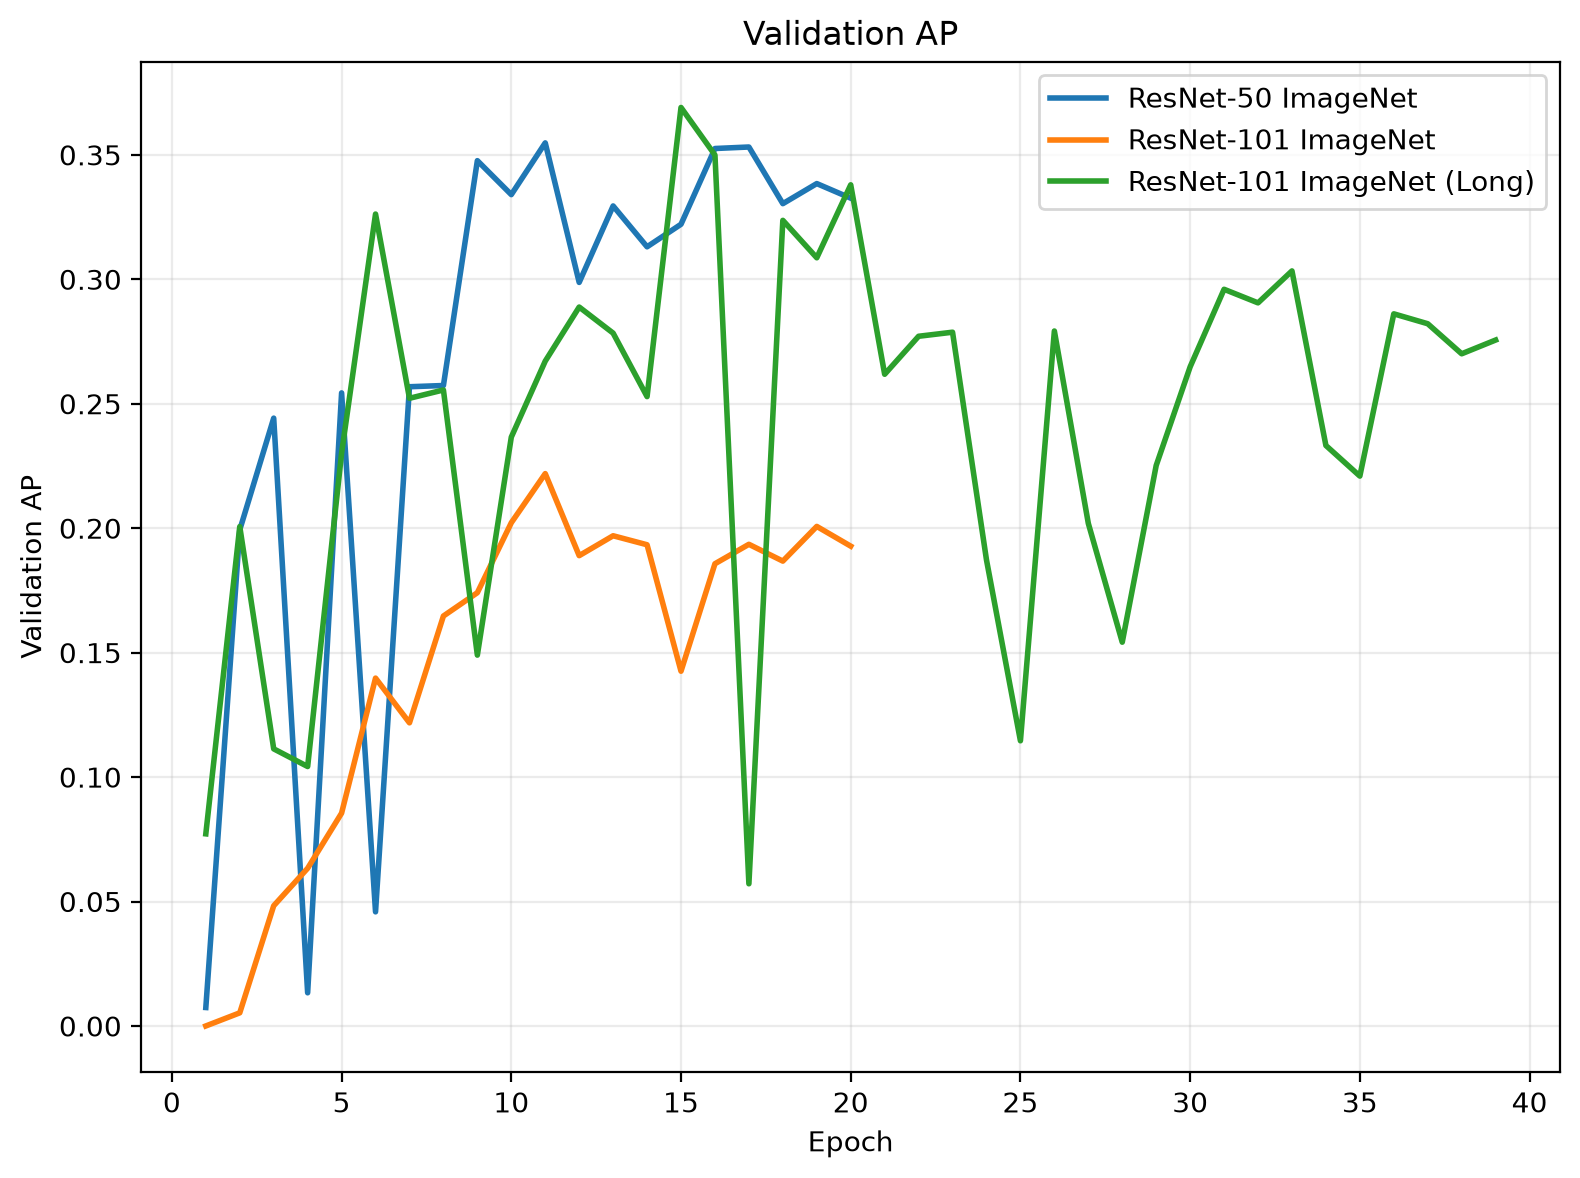
\includegraphics[width=0.6\textwidth]{Images/AP/why_long.png}
    \caption{Validation AP during development.}
    \label{fig:why_long}
\end{figure}

A first extended experiment showed that simply increasing the training time
while keeping the original optimization strategy did not provide a large
gain. The subsequent R101-IN recipe therefore changed several parameters at
the same time: the backbone was unfrozen earlier, warm-up was extended, the
batch size was increased from 8 to 16, and the backbone learning-rate factor
was raised from 0.1 to 0.3. The model was then fine-tuned starting from the
best checkpoint rather than from the final epoch of the main training phase.

This development process is relevant to the interpretation of the final
comparison. The four models do not have identical optimization histories,
even though they use the same detector architecture and evaluation pipeline.
The results should therefore be read as a comparison of the final systems
obtained under the available computational budget, rather than as a perfectly
controlled ablation of depth and initialization alone.


\subsection{Final Model Comparison}
\label{subsec:final_model_comparison}

The final detection results are reported in Table~\ref{tab:final_model_comparison}. R50-IN achieves the highest AP ($0.423$), followed by R50-CX ($0.399$) and R101-IN ($0.397$), while R101-CX reaches $0.239$. Increasing depth alone therefore does not guarantee higher AP. For all configurations, medium objects are considerably harder than large ones; the best $AP_M$ is $0.039$, compared with $AP_L=0.442$ for R50-IN.

\begin{table}[H]
    \centering
    \caption{Detection performance of the four final configurations.}
    \label{tab:final_model_comparison}
    \begin{tabular}{lcccccc}
        \hline
        \textbf{Model} & \textbf{AP} & \textbf{AP$_M$} & \textbf{AP$_L$} & \textbf{AR@10} & \textbf{AR$_M$} & \textbf{AR$_L$} \\
        \hline
        R50-CX & 0.399 & 0.024 & 0.433 & 0.876 & 0.904 & 0.981 \\
        R50-IN & \textbf{0.423} & \textbf{0.039} & \textbf{0.442} & 0.886 & 0.922 & 0.988 \\
        R101-CX & 0.239 & 0.029 & 0.231 & 0.804 & 0.920 & 0.974 \\
        R101-IN & 0.397 & 0.035 & 0.413 & \textbf{0.901} & \textbf{0.924} & \textbf{0.989} \\
        \hline
    \end{tabular}
\end{table}

R101-IN has the highest $AR@10$ ($0.901$), followed by R50-IN ($0.886$), and also gives the highest recall for medium and large objects. This is a useful complement to the AP ranking: the deeper ImageNet model recovers more ground-truth regions when up to ten detections are allowed, even though its confidence ranking is slightly less favourable overall. R101-CX has the lowest $AR@10$ ($0.804$), although its size-specific recall remains relatively high.

The difference between AP and AR is also visible in the size-specific results. All models perform much better on large regions than on medium ones, with $AP_M$ remaining below $0.04$ for every configuration. The limitation is therefore not restricted to a single backbone: small or medium annotated regions are intrinsically harder for the present detector.

The Precision--Recall curves in Figure~\ref{fig:precision_recall_comparison} confirm the AP ranking. R50-IN provides the strongest integrated precision--recall trade-off, while R101-CX remains below the other configurations over most of the recall range.

\begin{figure}[H]
    \centering
    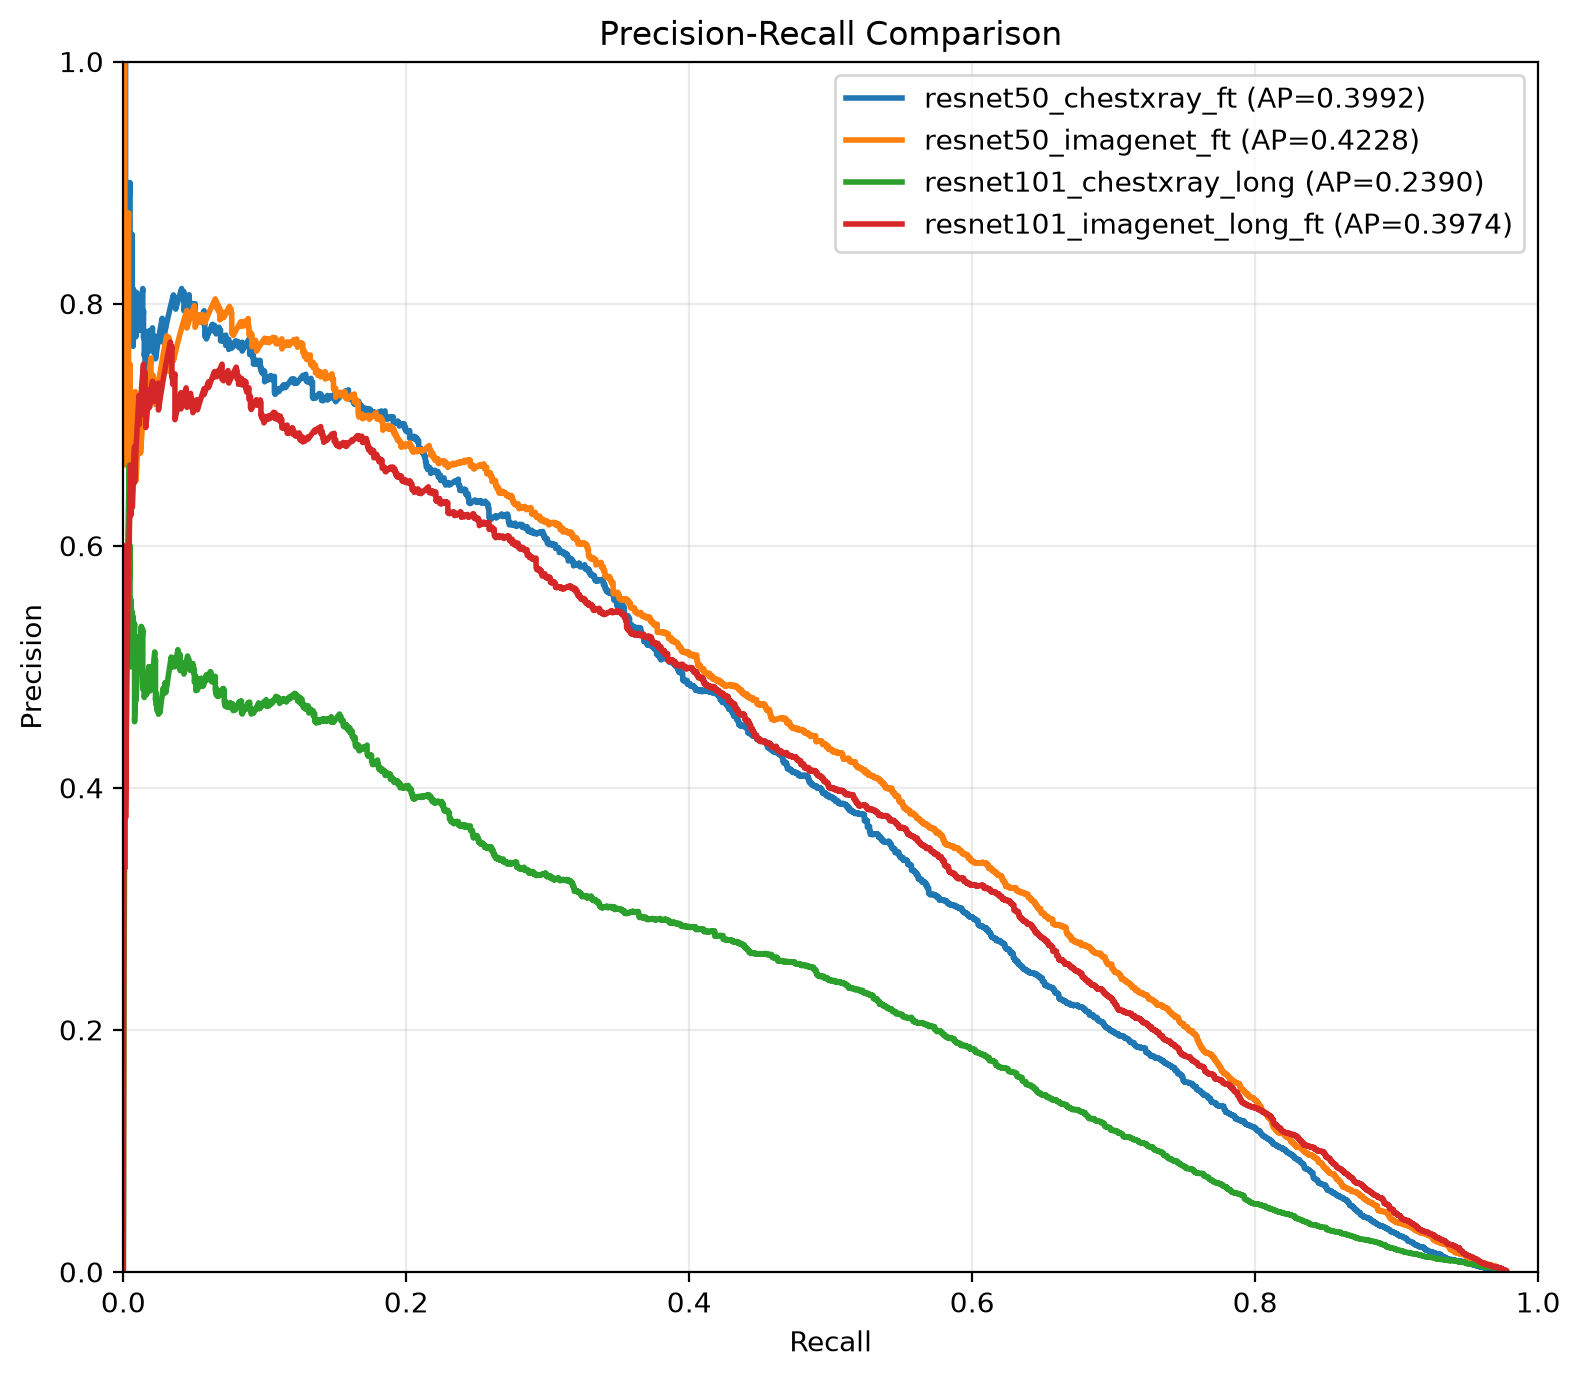
\includegraphics[width=0.6\textwidth]{Images/comparison/precision_recall_comparison.png}
    \caption{Precision--Recall curves.}
    \label{fig:precision_recall_comparison}
\end{figure}

\paragraph{Interpretation of the final comparison.}
The final results suggest that model depth mainly improves the ability to
recover annotated regions rather than automatically improving the integrated
precision--recall score. Moving from R50-IN to R101-IN increases $AR@10$ from
$0.886$ to $0.901$, while AP decreases slightly from $0.423$ to $0.397$. The
same pair also has very similar box-level F1 scores ($0.448$ and $0.446$).
This points to a difference in confidence ranking and detection behaviour
rather than a large difference in raw box localization quality.

The Chest-Xray initialization provides a useful contrast. R50-CX remains
close to the ImageNet models in several recall measures and reaches
$AP=0.399$, whereas R101-CX drops to $AP=0.239$. Since the final training
schedules were not identical, especially for the longer R101 experiments,
this result is better interpreted as a property of the complete training
pipelines than as an isolated measurement of pretraining quality.

\subsection{Operating-Point Analysis}
\label{subsec:operating_point}

The model-specific operating points are reported in Table~\ref{tab:operating_point_comparison}. The selected thresholds are close ($0.36$--$0.41$), so the differences are not simply due to very different confidence regions. R101-IN is strongest at this operating point, with precision $0.552$, recall $0.846$, specificity $0.800$, F1 $0.668$ and Youden $J=0.646$.

\begin{table}[H]
    \centering
    \caption{Image-level performance at the Youden operating point.}
    \label{tab:operating_point_comparison}
    \begin{tabular}{lcccccc}
        \hline
        \textbf{Model} & $\boldsymbol{\tau^*}$ & \textbf{Precision} & \textbf{Recall} & \textbf{Specificity} & \textbf{F1} & \textbf{Youden J} \\
        \hline
        R50-CX & 0.36 & 0.508 & 0.838 & 0.764 & 0.633 & 0.602 \\
        R50-IN & 0.39 & 0.535 & 0.840 & 0.788 & 0.654 & 0.628 \\
        R101-CX & 0.38 & 0.535 & 0.824 & 0.792 & 0.649 & 0.616 \\
        R101-IN & 0.41 & \textbf{0.552} & \textbf{0.846} & \textbf{0.800} & \textbf{0.668} & \textbf{0.646} \\
        \hline
    \end{tabular}
\end{table}

The corresponding confusion matrices are shown in Figure~\ref{fig:confusion_matrices}. R101-IN produces the largest number of true positives ($1017$) and true negatives ($3307$), as well as the fewest false positives ($827$). These results also illustrate why AP and image-level F1 need not give the same ranking.

\begin{figure}[H]
    \centering
    \begin{minipage}{0.48\textwidth}
        \centering
        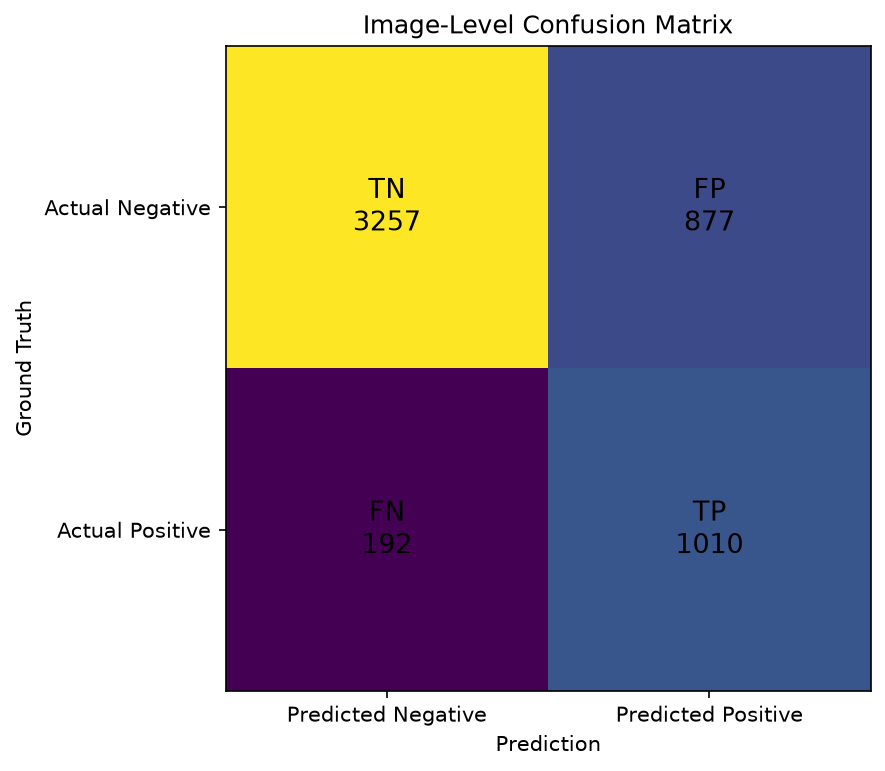
\includegraphics[width=\textwidth]{Images/confusion_matrix/resnet50_imagenet_ft.png}
        \caption*{(a) R50-IN}
    \end{minipage}
    \hfill
    \begin{minipage}{0.48\textwidth}
        \centering
        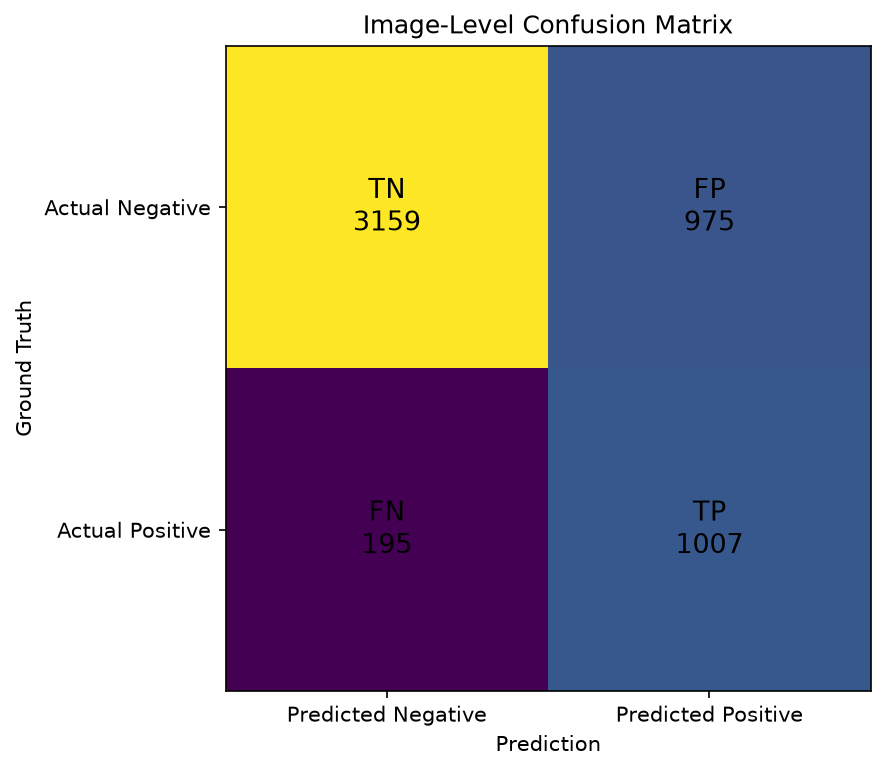
\includegraphics[width=\textwidth]{Images/confusion_matrix/resnet50_chestxray_ft.png}
        \caption*{(b) R50-CX}
    \end{minipage}

    \vspace{0.35cm}

    \begin{minipage}{0.48\textwidth}
        \centering
        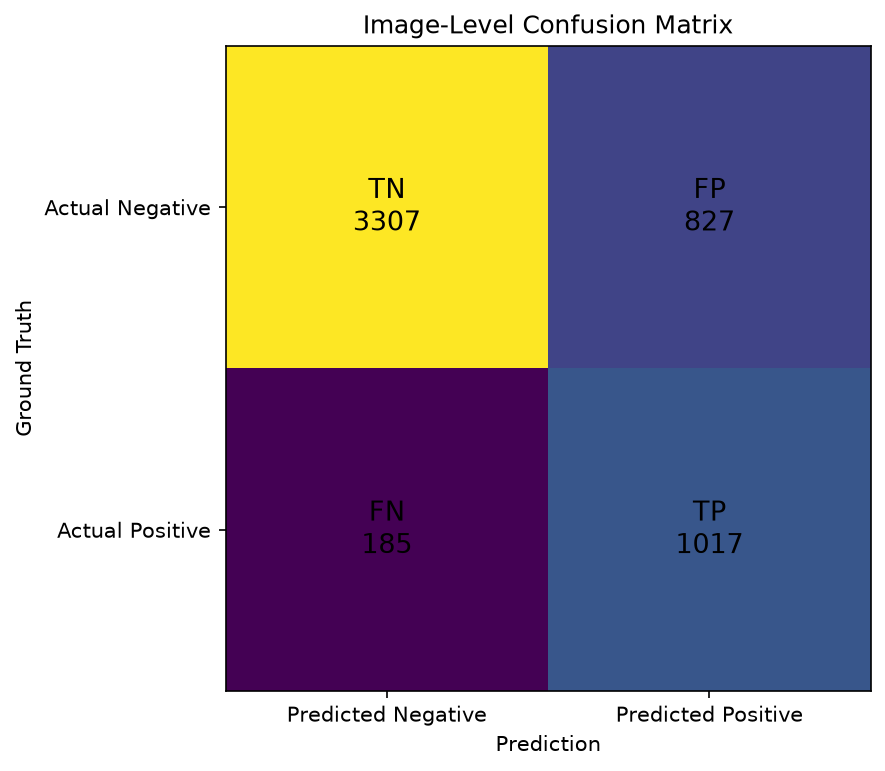
\includegraphics[width=\textwidth]{Images/confusion_matrix/resnet101_imagenet_long_ft.png}
        \caption*{(c) R101-IN}
    \end{minipage}
    \hfill
    \begin{minipage}{0.48\textwidth}
        \centering
        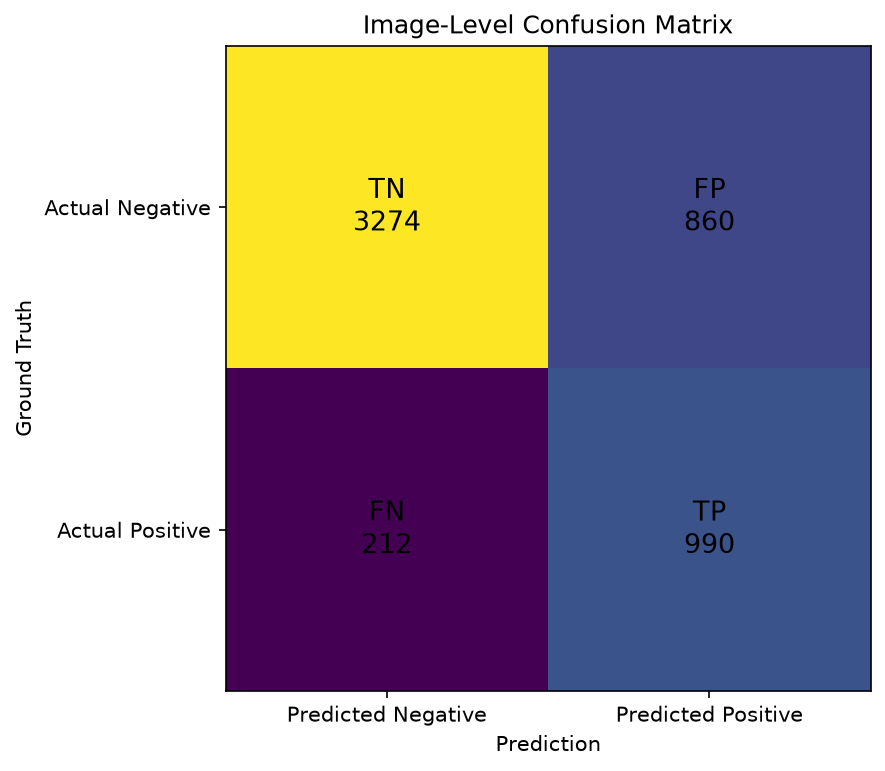
\includegraphics[width=\textwidth]{Images/confusion_matrix/resnet101_chestxray_long.png}
        \caption*{(d) R101-CX}
    \end{minipage}

    \caption{Confusion matrices at the Youden operating points.}
    \label{fig:confusion_matrices}
\end{figure}

\subsection{Localization Analysis}
\label{subsec:localization}

The mean matched IoU is $0.684$, $0.688$, $0.659$ and $0.692$ for R50-CX, R50-IN, R101-CX and R101-IN, respectively. R101-IN therefore gives the highest average overlap. Box-level F1 is $0.424$, $0.448$, $0.388$ and $0.446$, showing that the two ImageNet configurations are close at box level.

\begin{figure}[H]
    \centering
    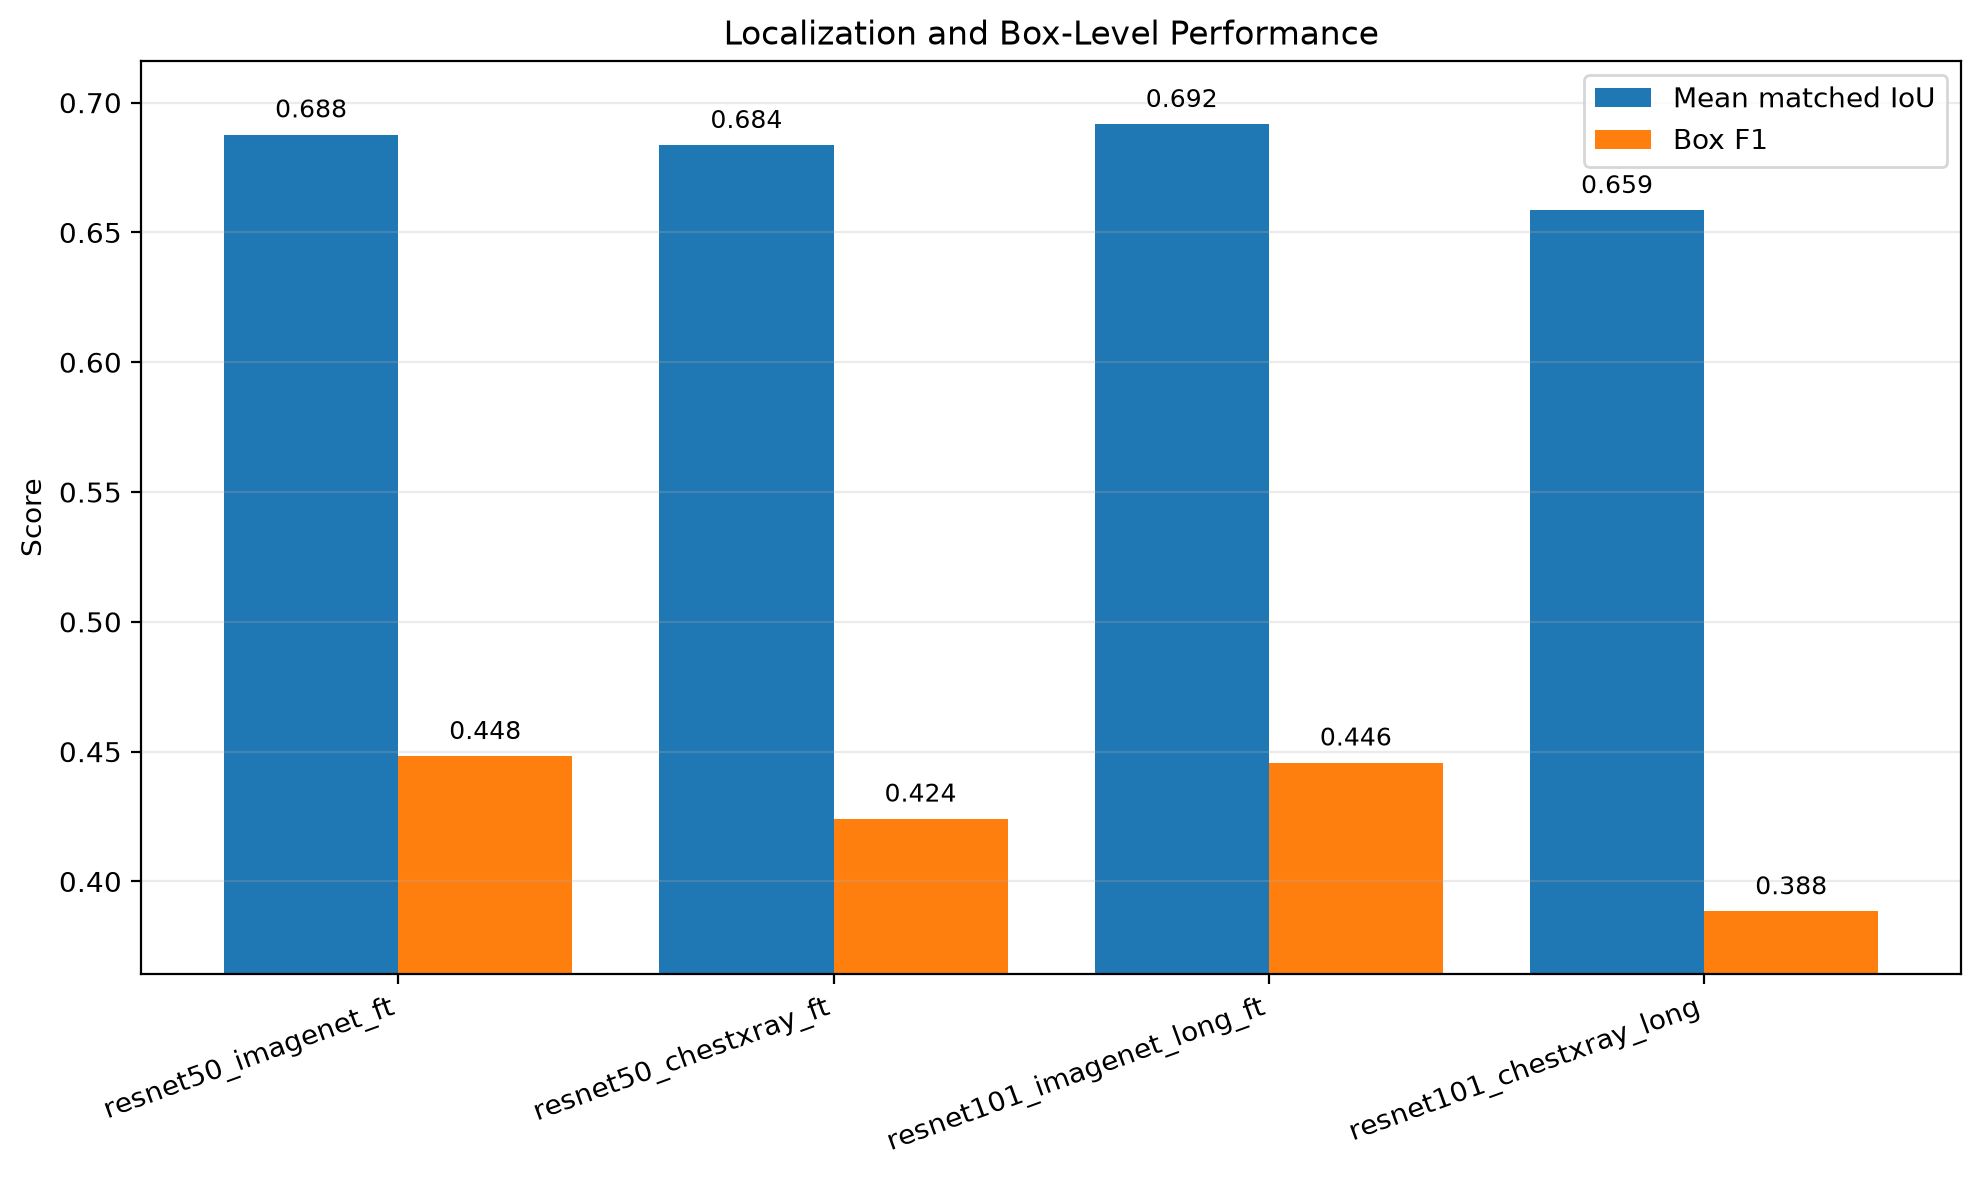
\includegraphics[width=0.6\textwidth]{Images/comparison/localization_comparison.png}
    \caption{Localization metrics at the Youden operating points.}
    \label{fig:localization_comparison}
\end{figure}

R101-IN's lower AP does not correspond to poorer localization: it combines the highest mean matched IoU with the highest image-level recall, while R50-IN remains preferable when integrated AP is the main criterion.

\subsection{Qualitative Analysis}
\label{subsec:qualitative}

The qualitative examples are evaluated at the model-specific Youden thresholds
and illustrate both image-level and localization disagreement. In
Figure~\ref{fig:qualitative_category}, (a) R101-CX misses the case while the
other configurations detect it, whereas in (b) both ImageNet-initialized
models miss the annotated target while the Chest-Xray-initialized models
detect it. The localization examples in
Figure~\ref{fig:qualitative_localization} show that, even when the image-level
decision agrees, the predicted boxes can differ in number, size, and position.

These examples highlight two complementary aspects of detector behaviour.
Image-level disagreement reflects whether a prediction is retained at all,
whereas localization disagreement concerns differences in the spatial extent
and position of the predicted boxes. This supports the use of both detection
metrics and box-level analysis when comparing the four configurations.

\begin{figure}[H]
    \centering
    \subfloat[R101-CX misses the case; the other configurations detect it.]{%
        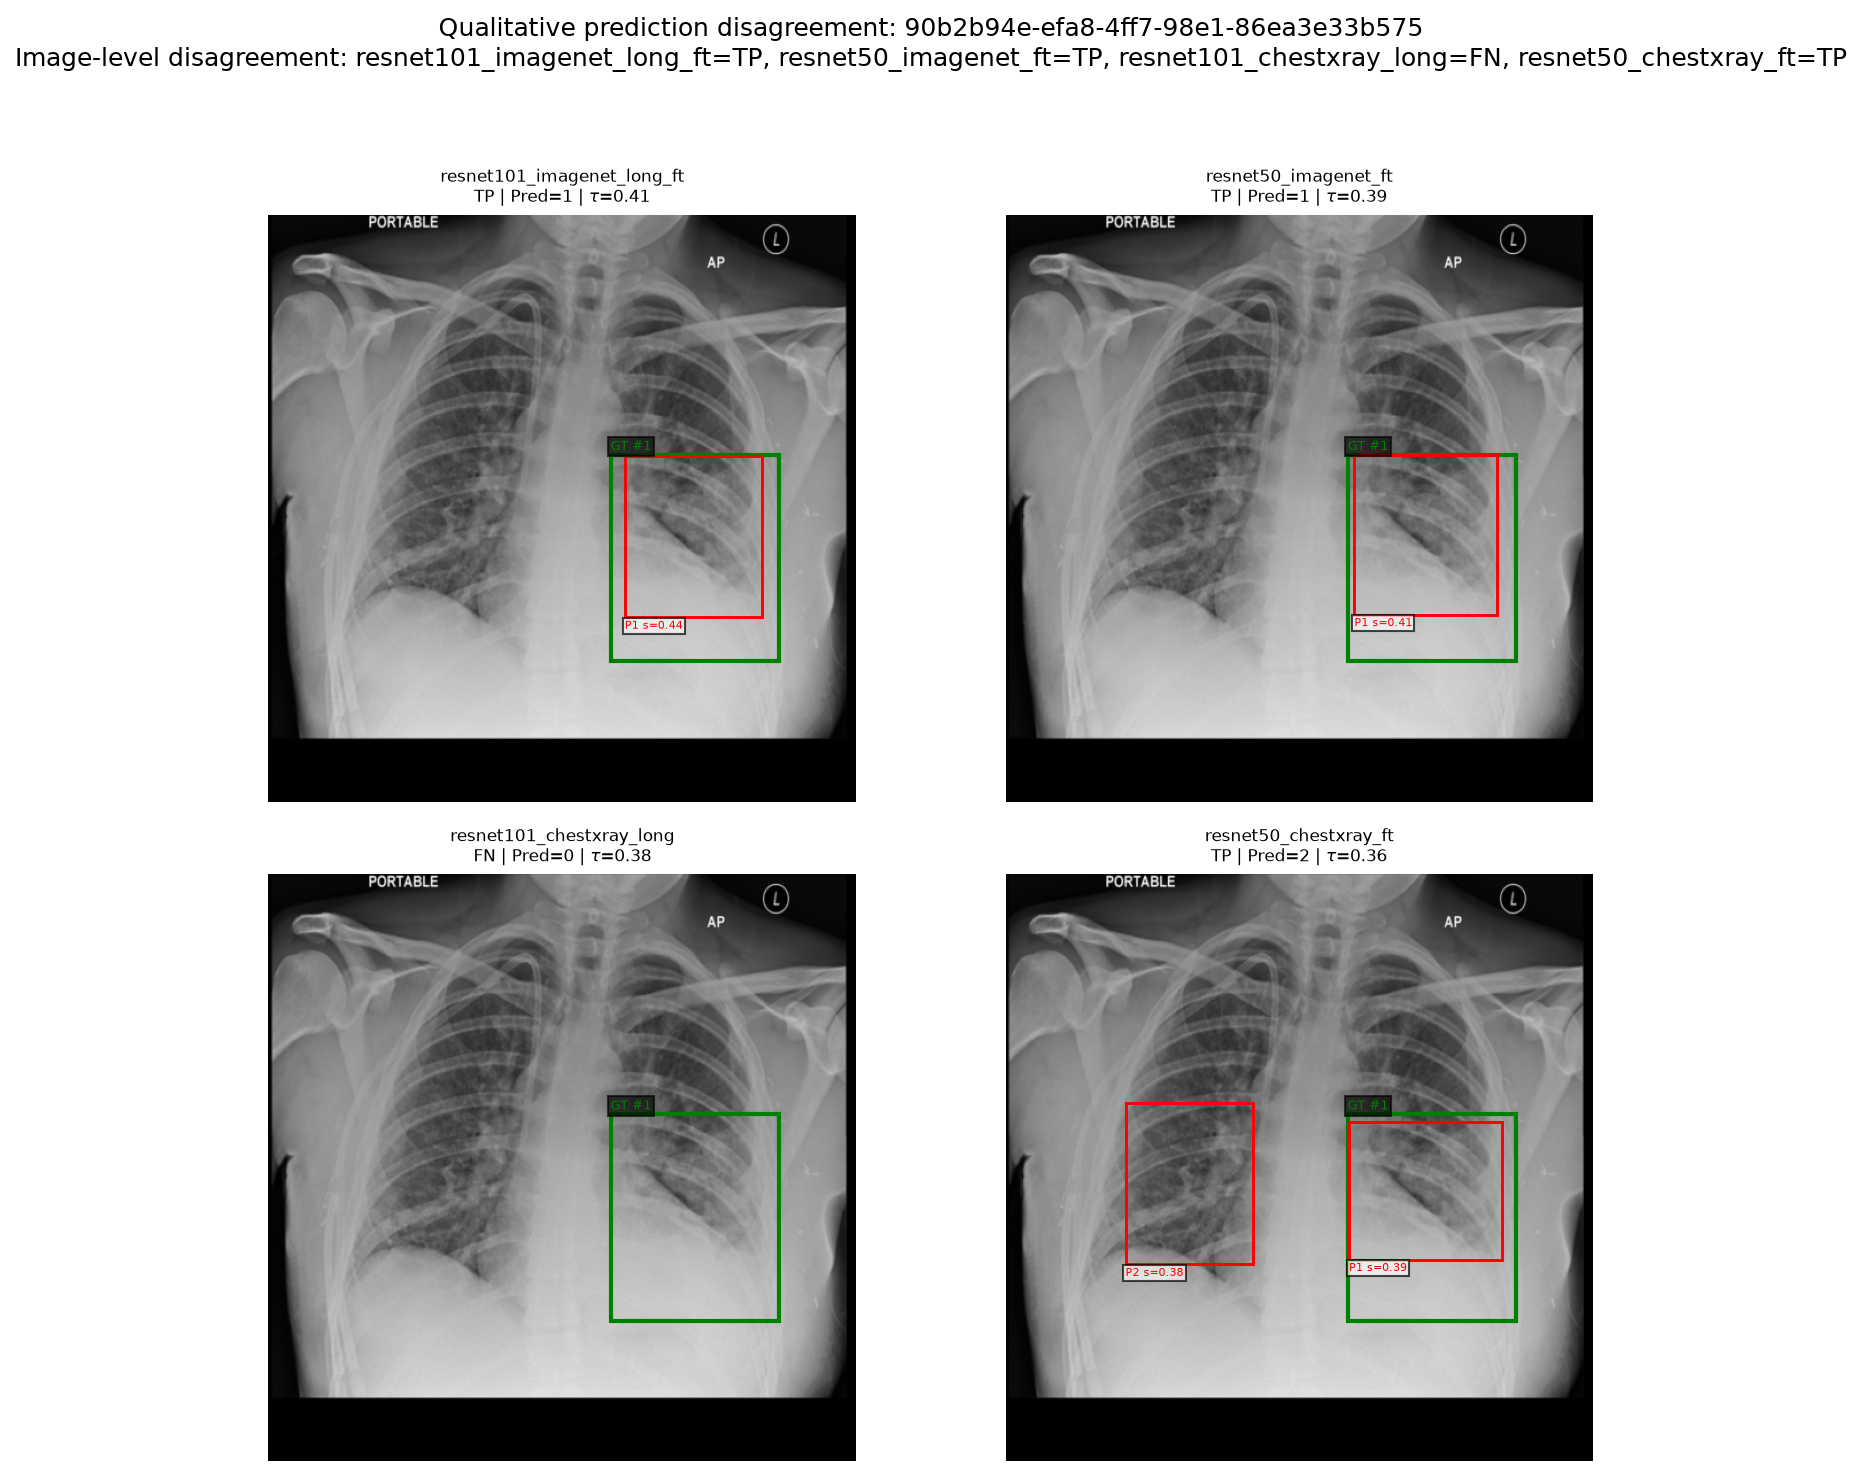
\includegraphics[width=0.47\textwidth]{Images/qualitative/qualitative_90b2b94e.png}%
    }
    \hfill
    \subfloat[ImageNet models miss the target; Chest-Xray models detect it.]{%
        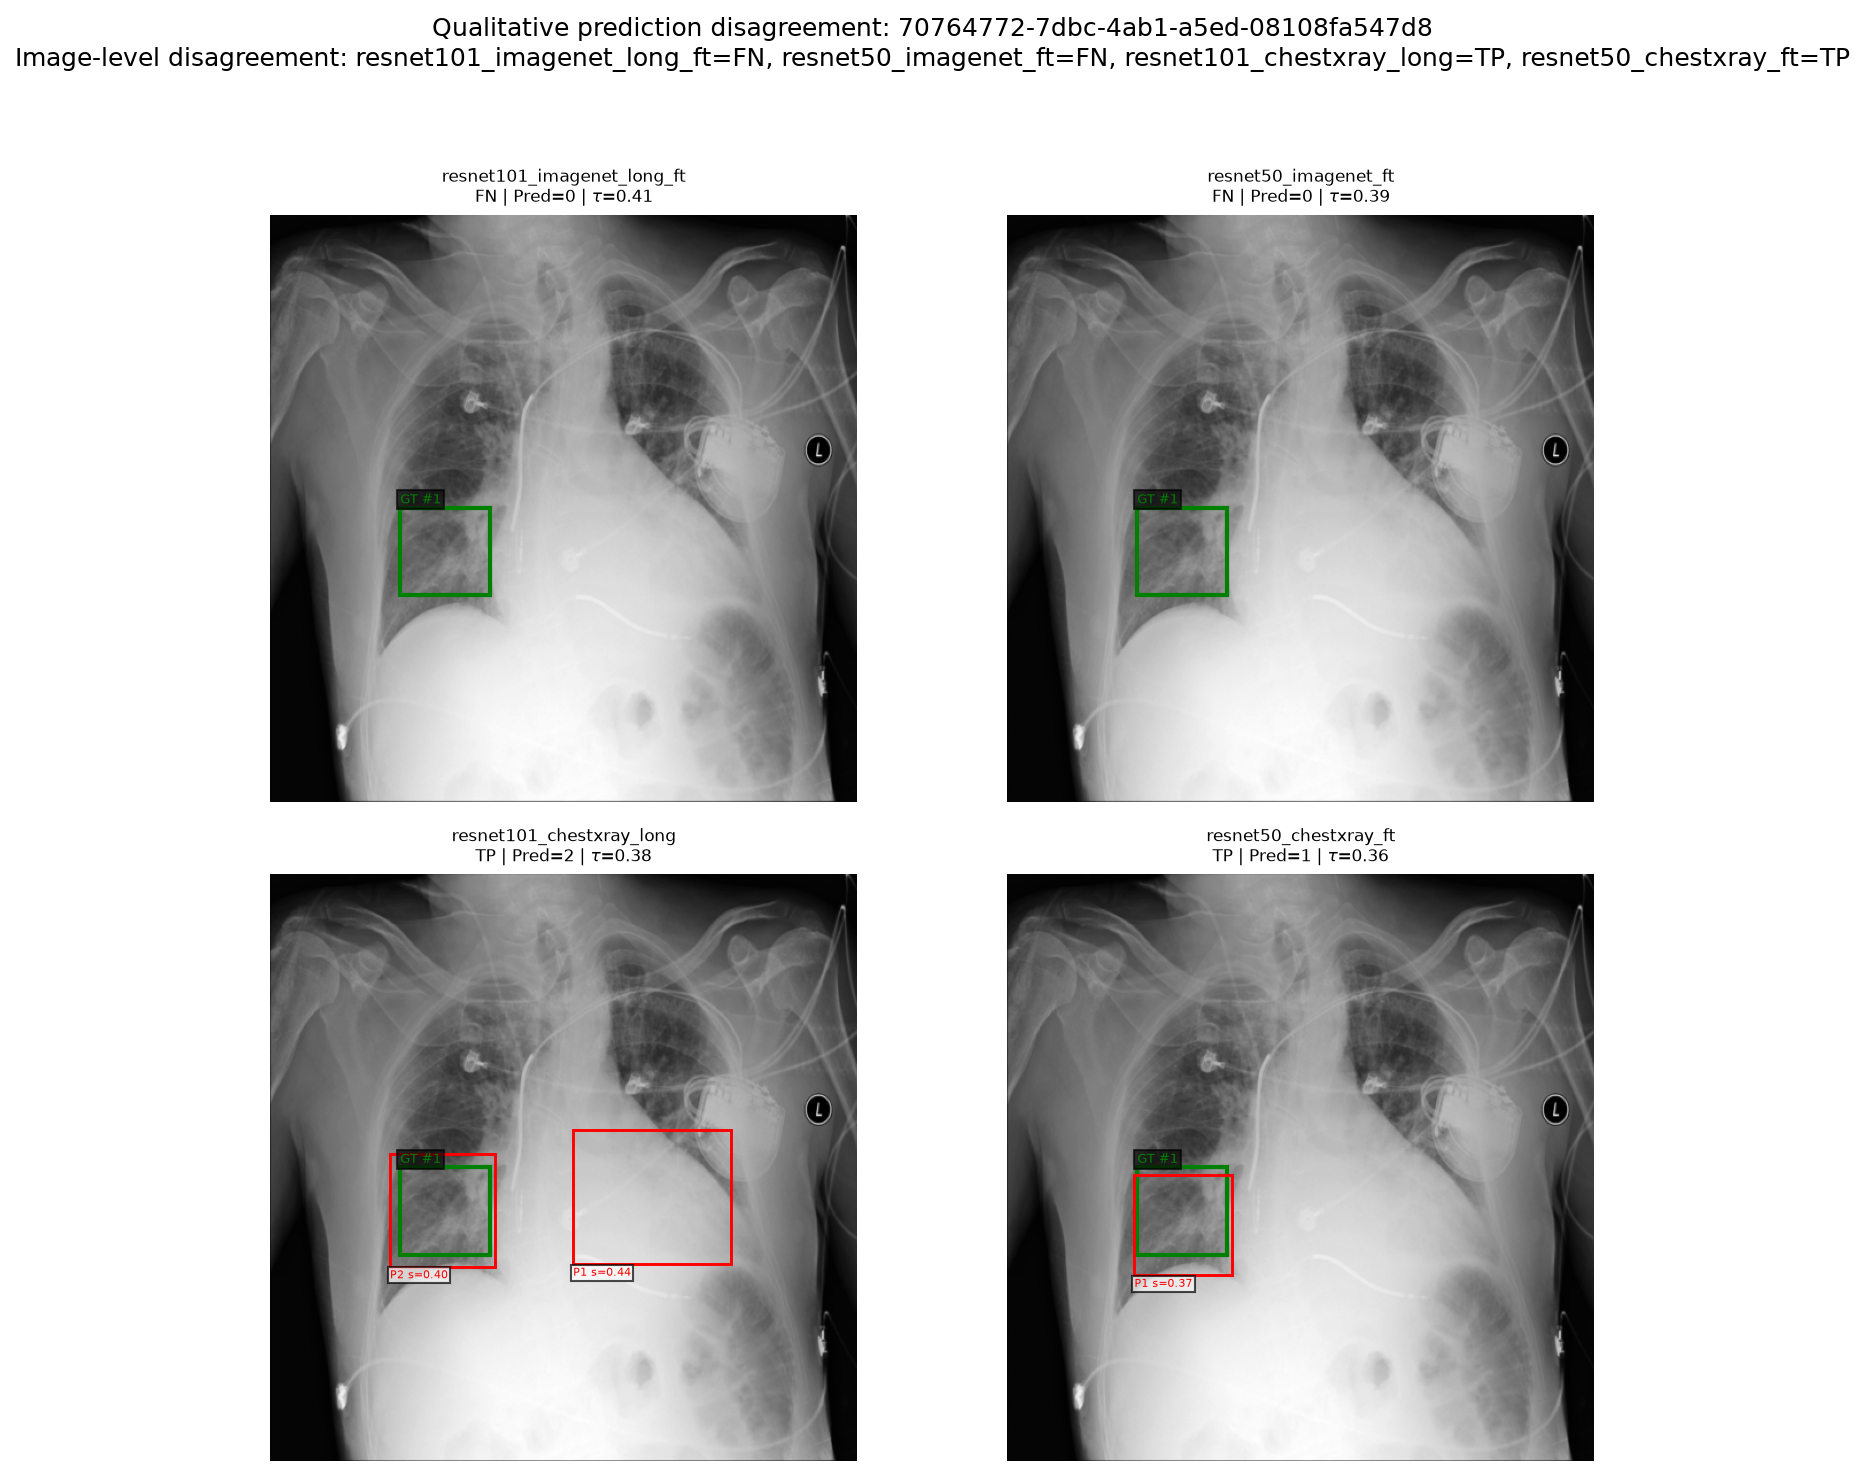
\includegraphics[width=0.47\textwidth]{Images/qualitative/qualitative_70764772.png}%
    }
    \caption{Representative image-level prediction disagreements. Green:
    ground truth; red: predictions.}
    \label{fig:qualitative_category}
\end{figure}

\begin{figure}[H]
    \centering
    \subfloat[Localization disagreement case 1]{%
        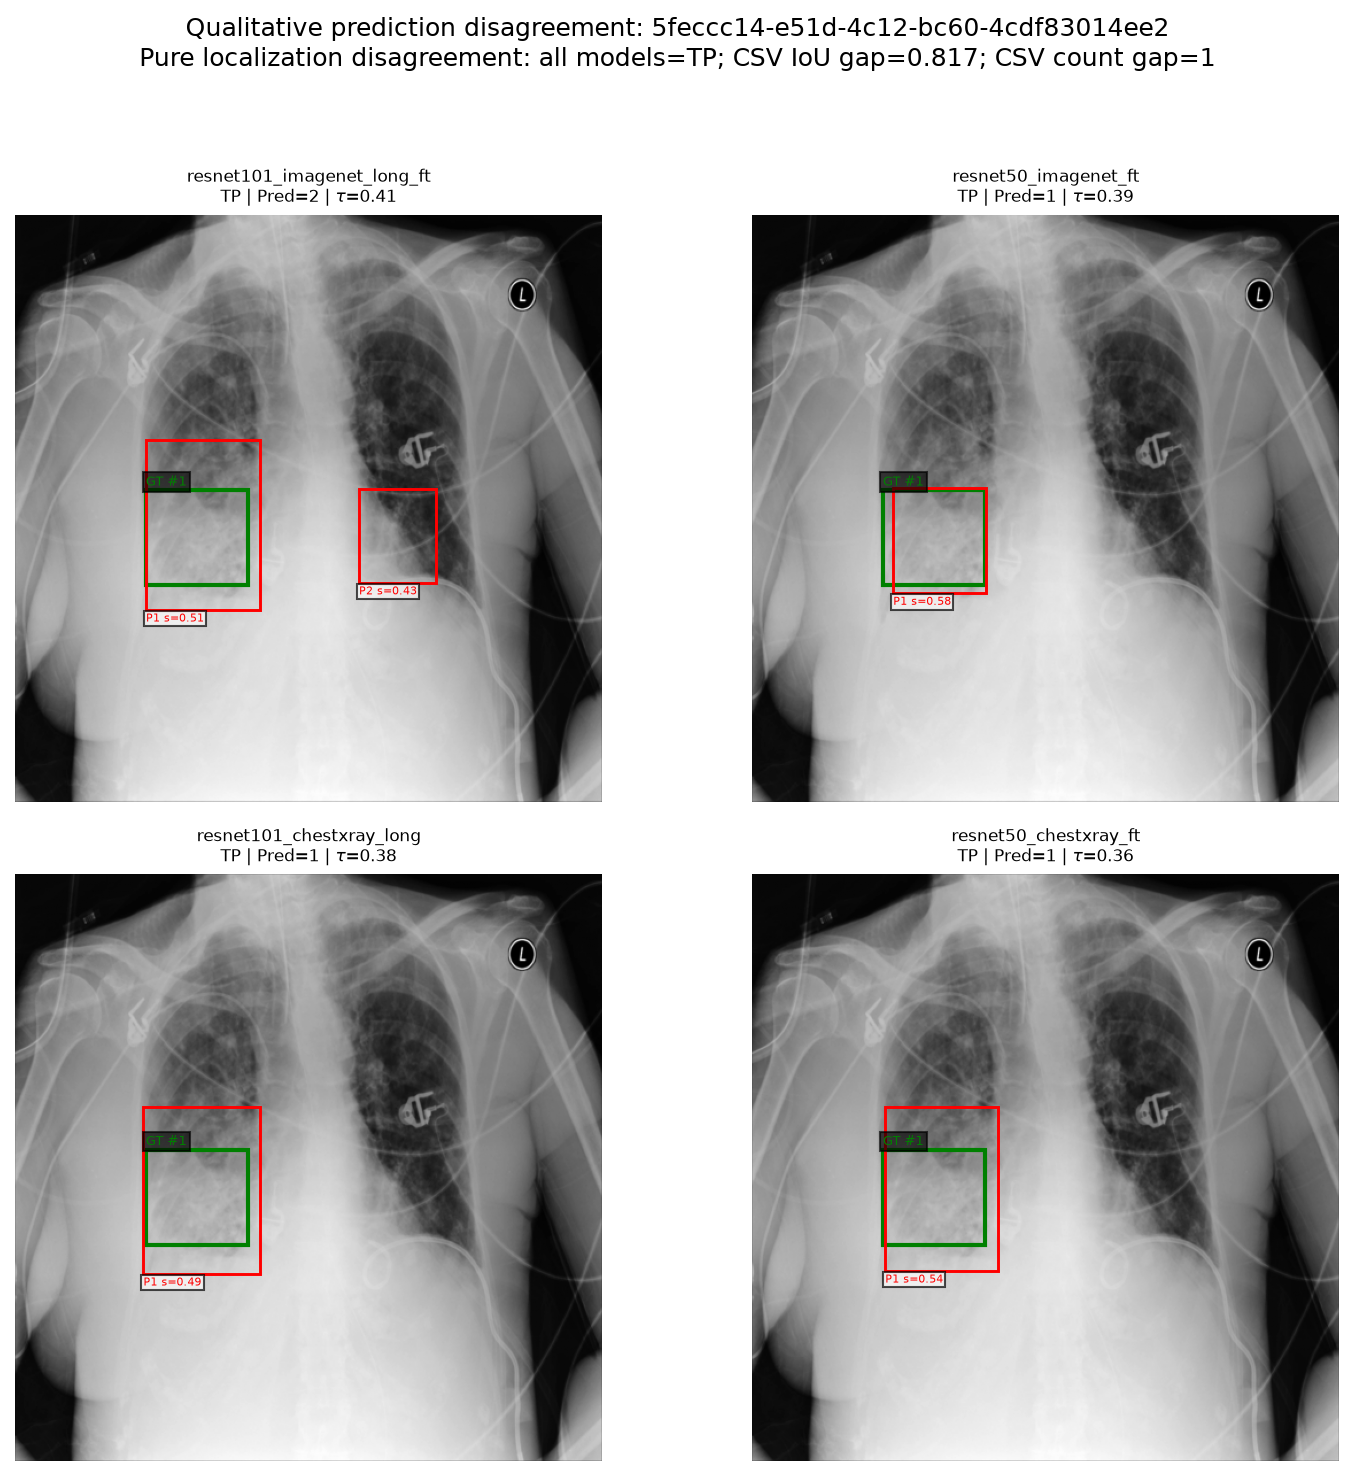
\includegraphics[width=0.47\textwidth]{Images/qualitative/qualitative_5feccc14.png}%
    }
    \hfill
    \subfloat[Localization disagreement case 2]{%
        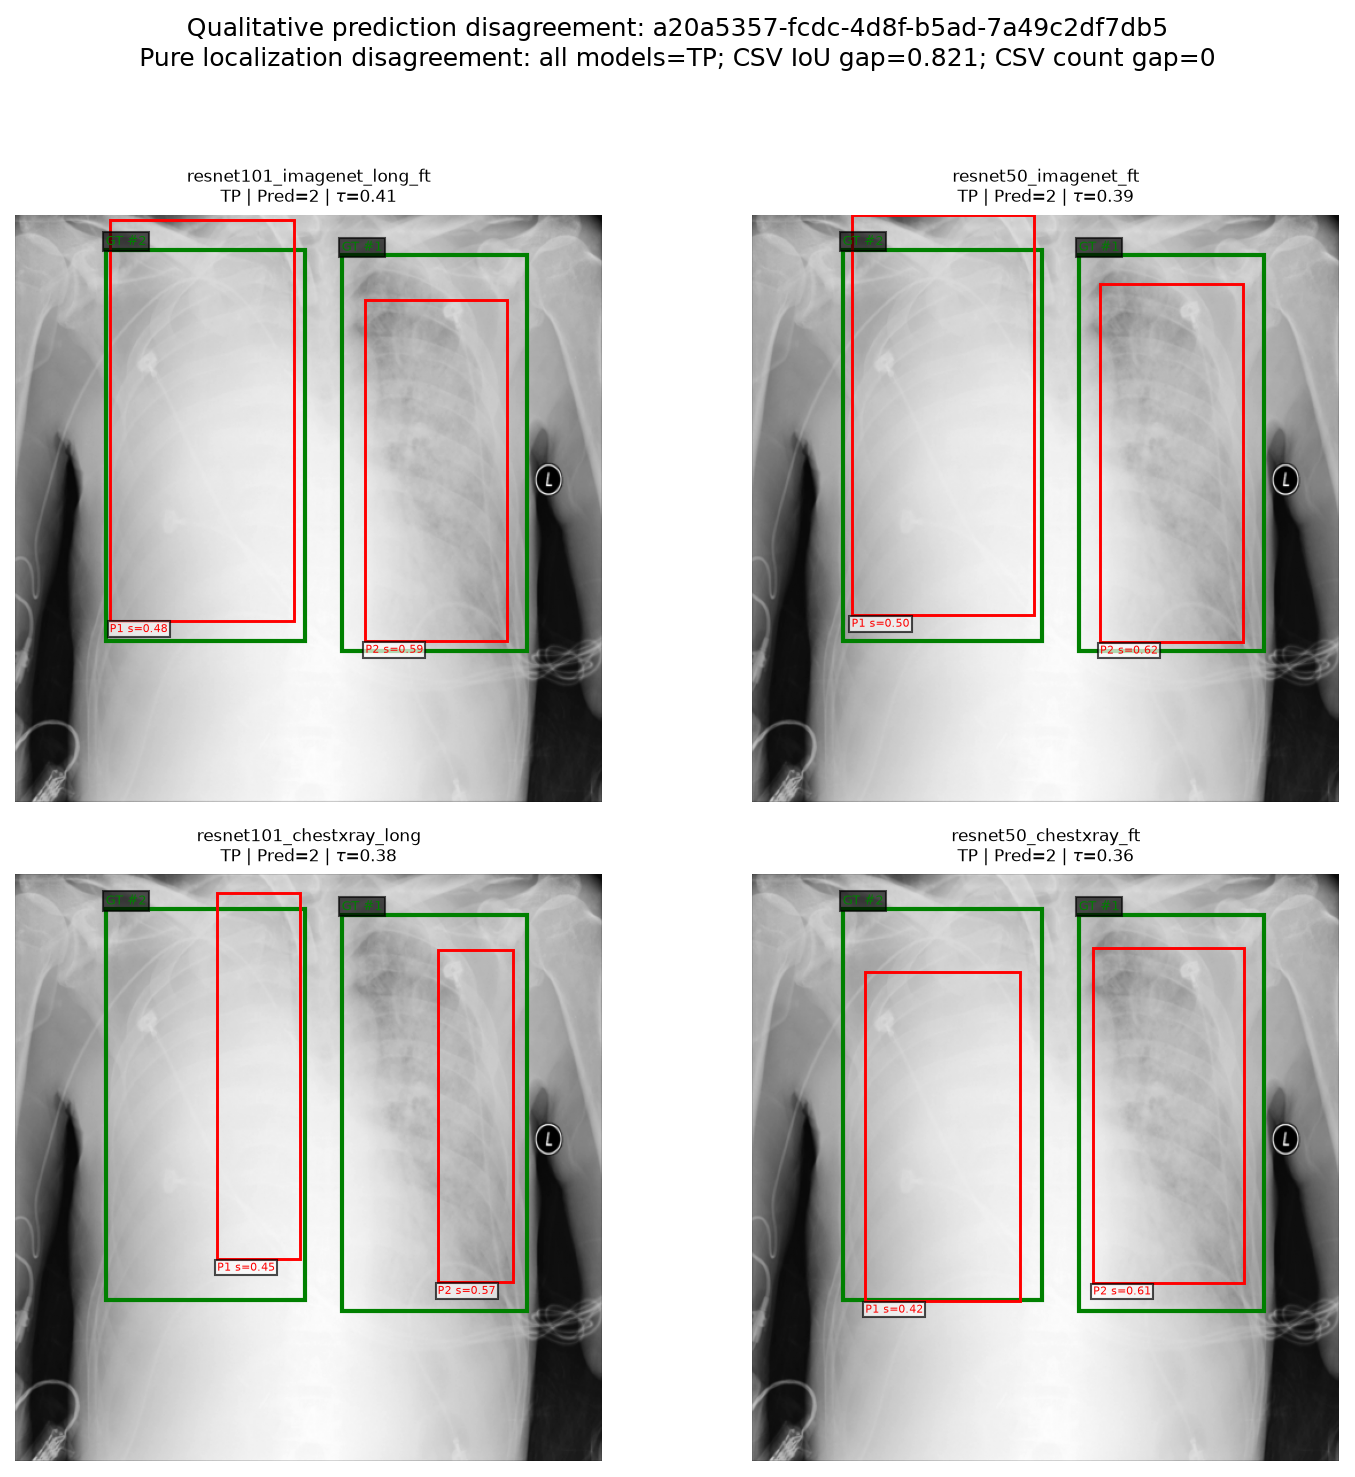
\includegraphics[width=0.47\textwidth]{Images/qualitative/qualitative_a20a5357.png}%
    }
    \caption{Representative localization disagreements. Green: ground truth;
    red: predictions.}
    \label{fig:qualitative_localization}
\end{figure}

\subsection{Additional Visualizations}
\label{subsec:additional_visualizations}

Additional qualitative visualizations are provided to complement the
quantitative results and illustrate both the intermediate feature
representations and the final detector predictions.

\subsubsection{Feature Flow}
\label{subsubsec:feature_flow}

The same input radiograph is passed through the four final configurations,
and the resulting feature flow through the backbone and FPN is visualized in
Figure~\ref{fig:feature_flow_comparison}. These representations are intended
for qualitative comparison and do not provide a direct performance measure.

\begin{figure}[H]
    \centering
    \subfloat[R50-CX]{%
        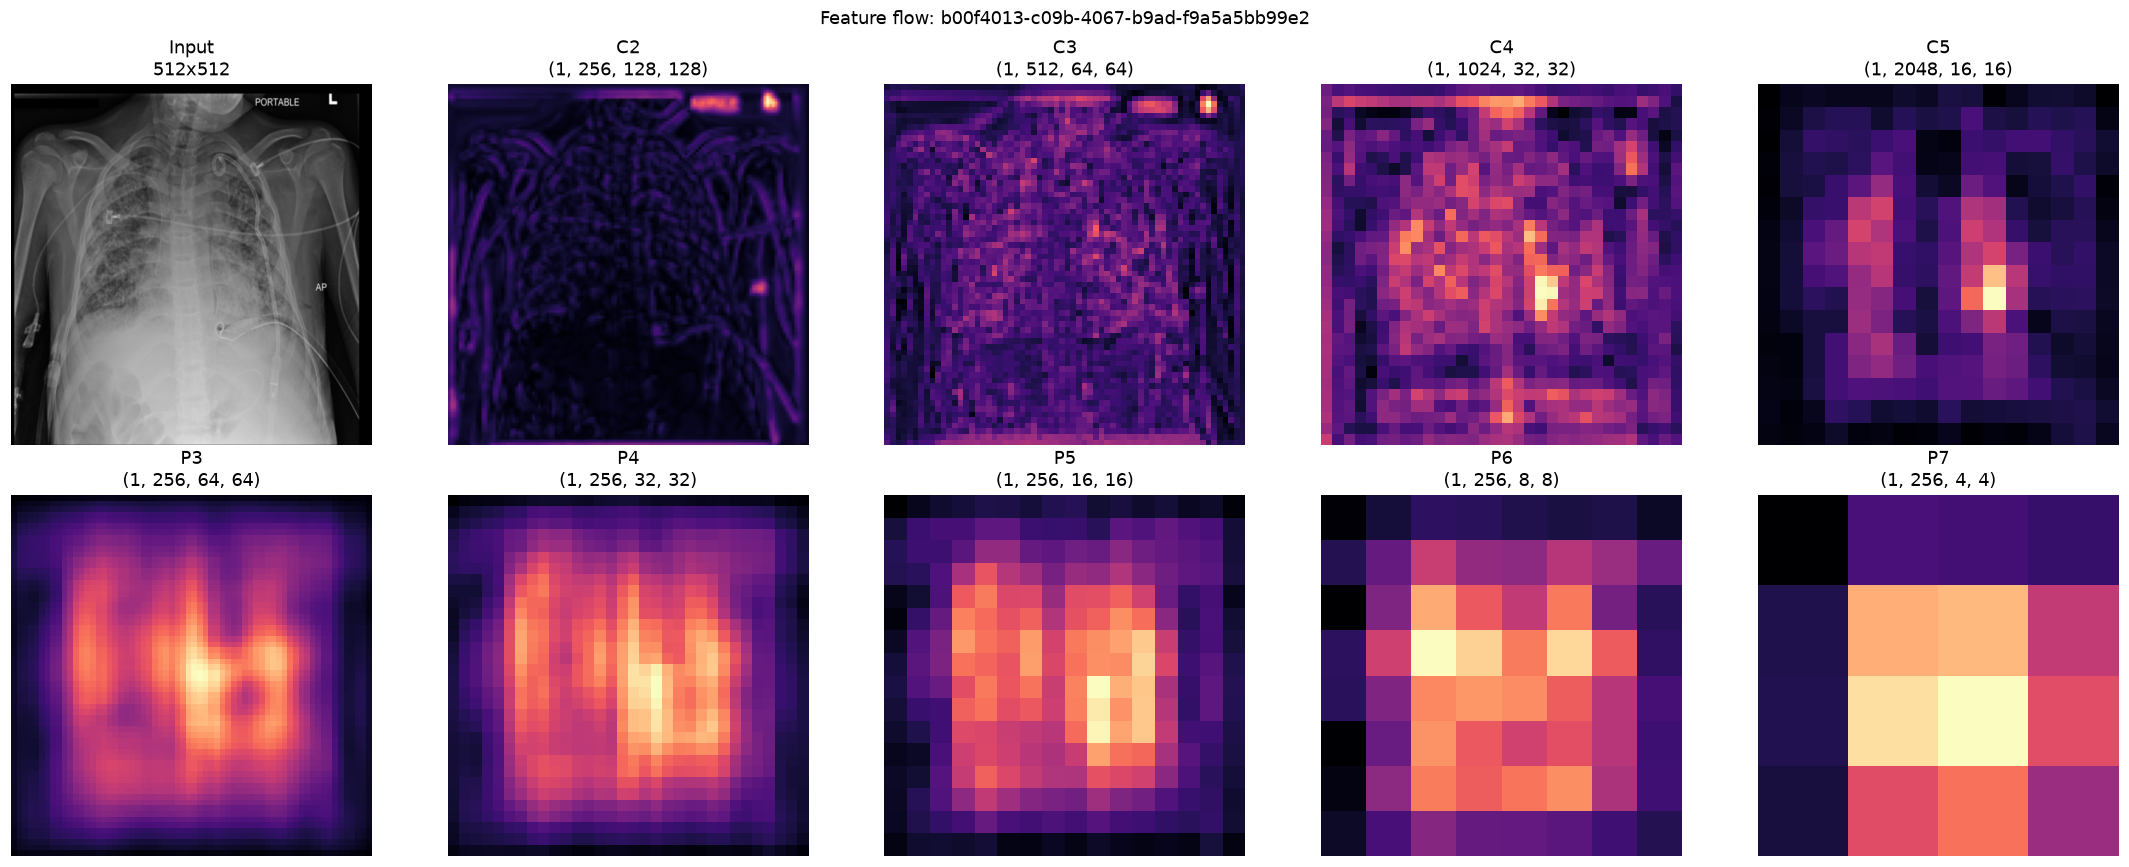
\includegraphics[width=0.47\textwidth]{Images/qualitative/feature_flow_r50_cx.png}%
    }
    \hfill
    \subfloat[R50-IN]{%
        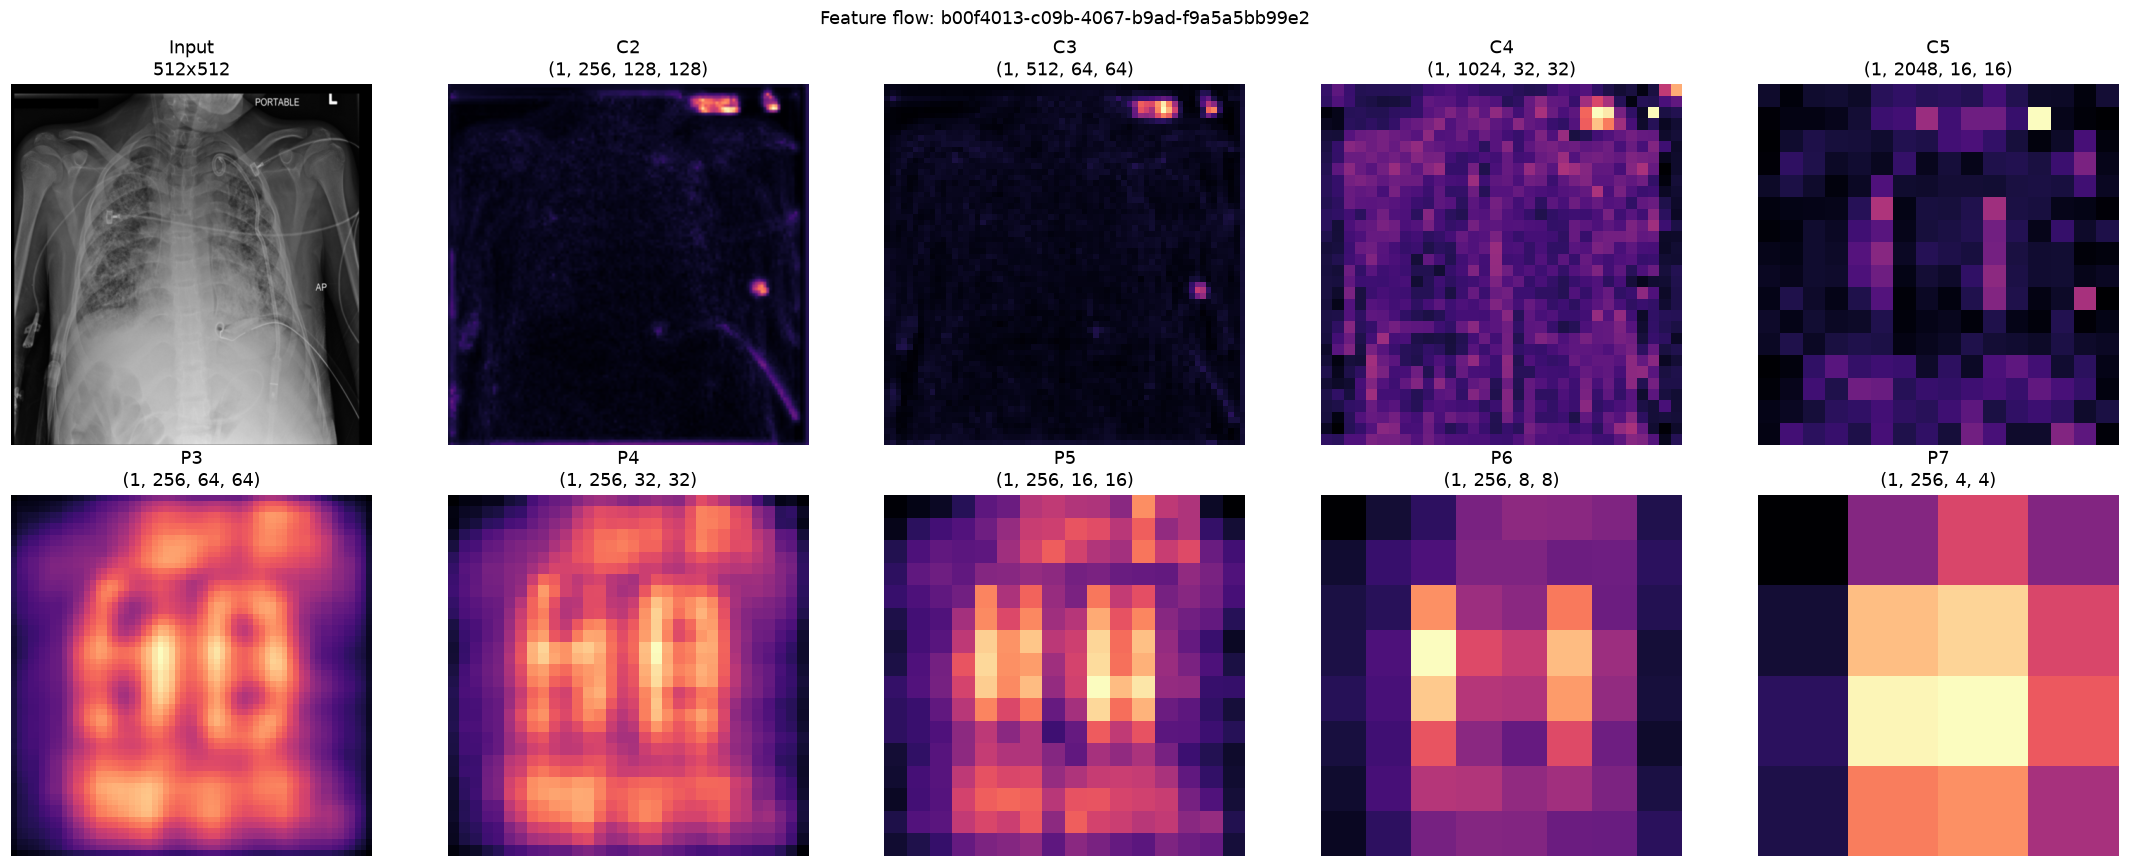
\includegraphics[width=0.47\textwidth]{Images/qualitative/feature_flow_r50_in.png}%
    }

    \vspace{0.35cm}

    \subfloat[R101-CX]{%
        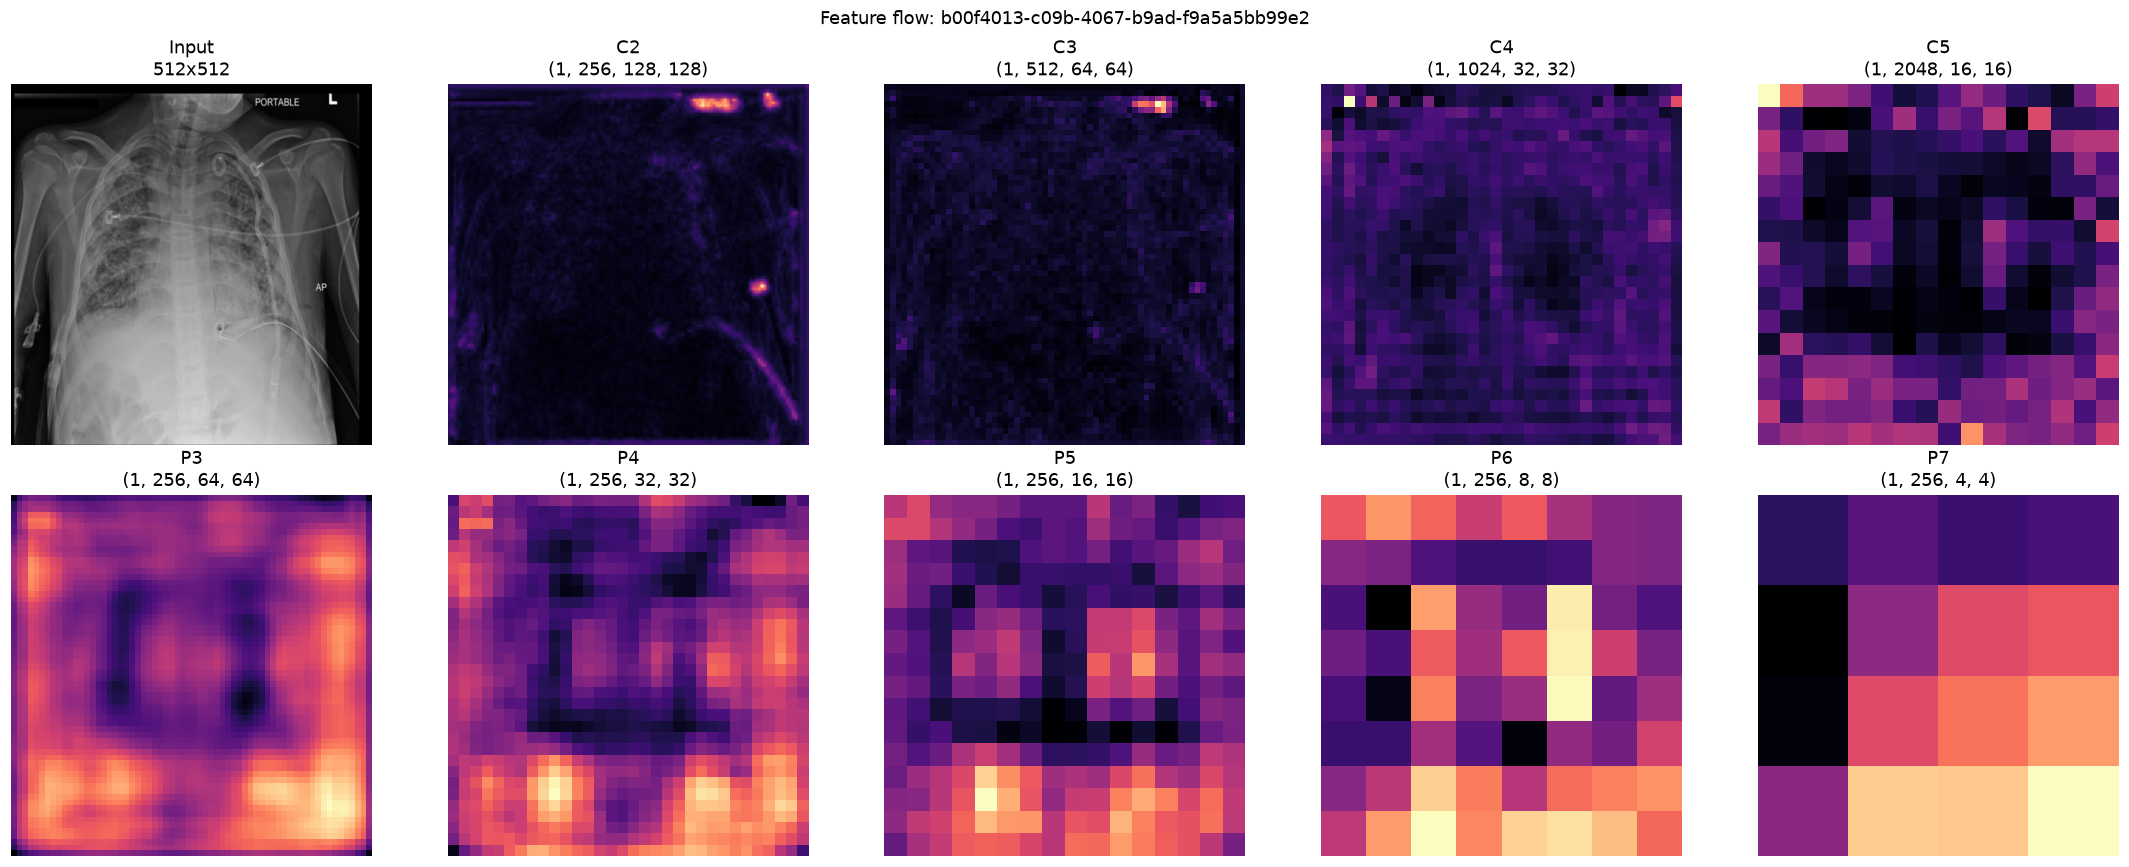
\includegraphics[width=0.47\textwidth]{Images/qualitative/feature_flow_r101_cx.png}%
    }
    \hfill
    \subfloat[R101-IN]{%
        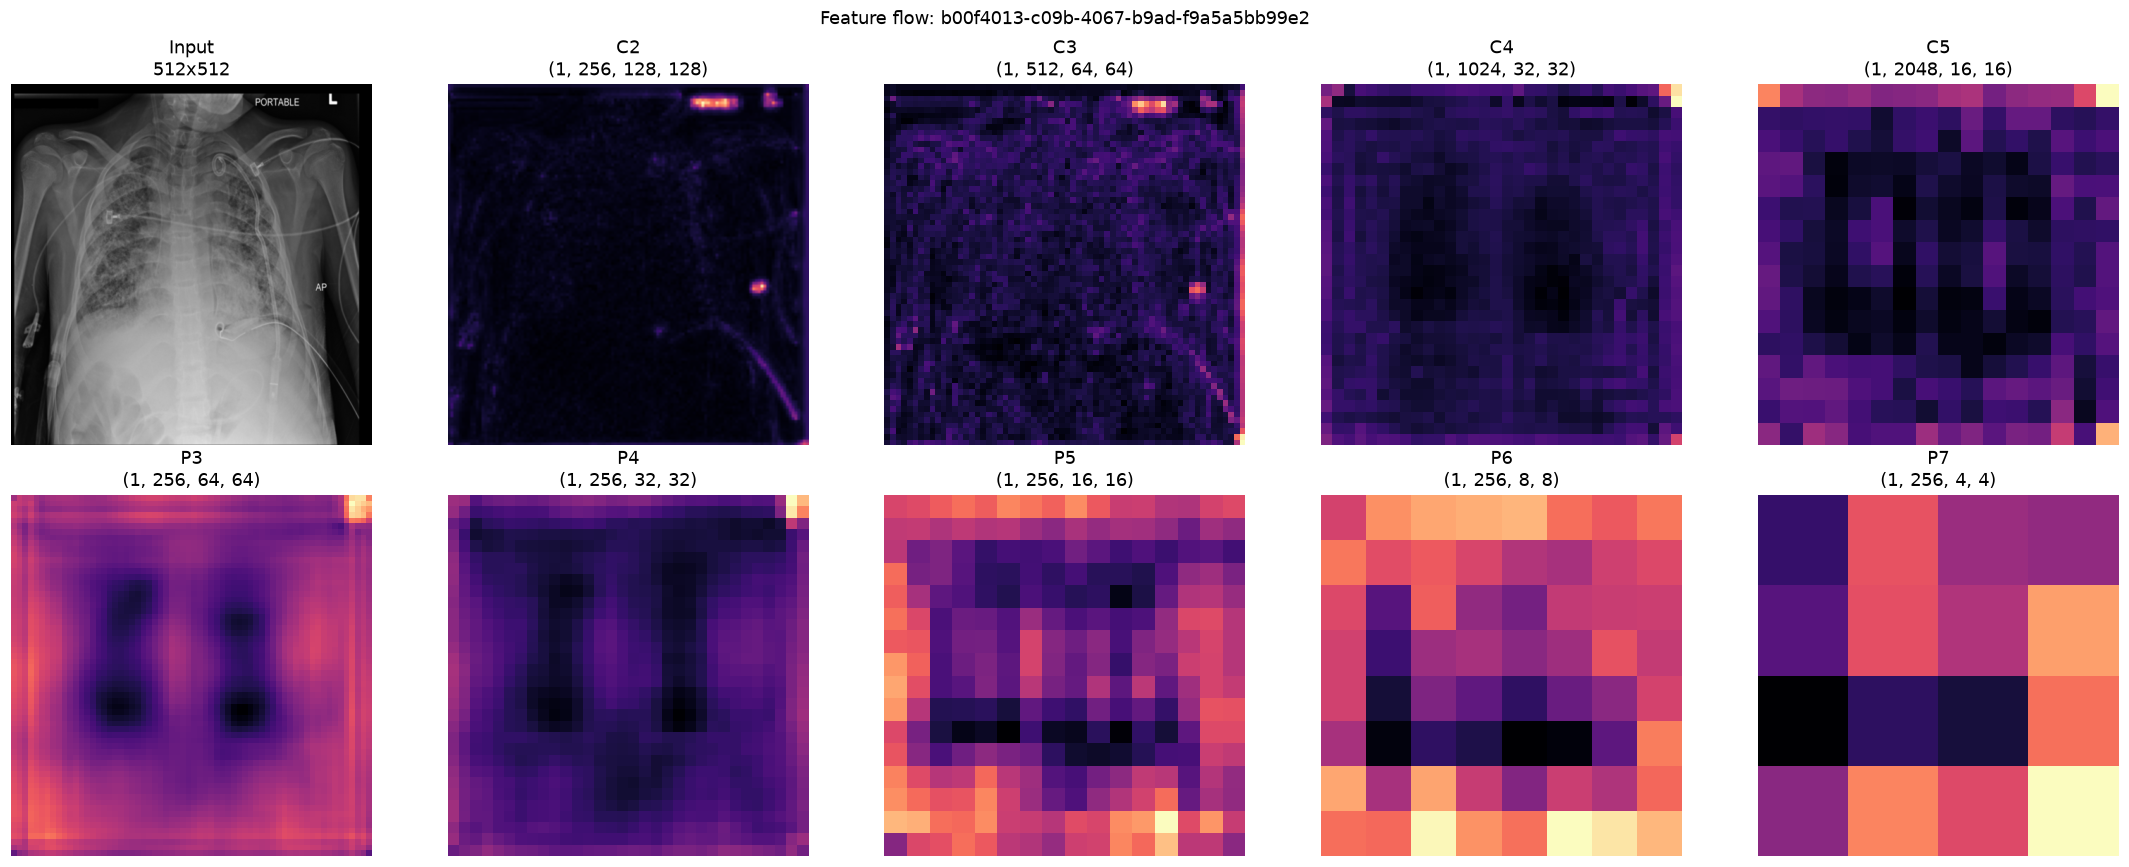
\includegraphics[width=0.47\textwidth]{Images/qualitative/feature_flow_r101_in.png}%
    }
    \caption{Feature flow for the four final detector configurations on the same input image.}
    \label{fig:feature_flow_comparison}
\end{figure}

\subsubsection{Representative Detections}
\label{subsubsec:representative_detections}

Figures~\ref{fig:representative_detections_case1}
and~\ref{fig:representative_detections_case2}
show representative predictions from the two ImageNet-initialized
configurations, R50-IN and R101-IN, selected
as the strongest overall models in the quantitative comparison.

\begin{figure}[H]
    \centering
    \subfloat[R50-IN -- case 1]{%
        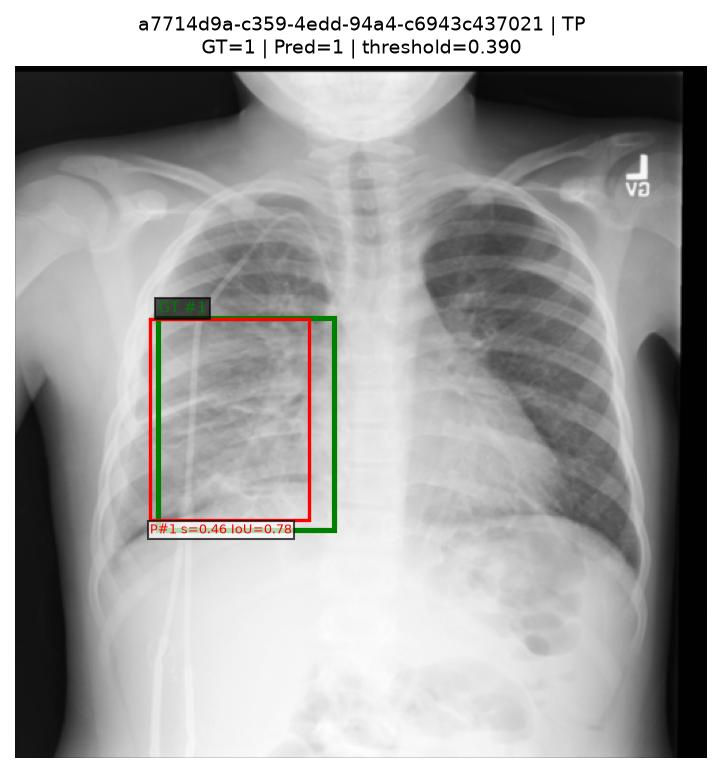
\includegraphics[width=0.45\textwidth]{Images/qualitative/r50_in_case1.jpg}%
    }
    \hfill
    \subfloat[R101-IN -- case 1]{%
        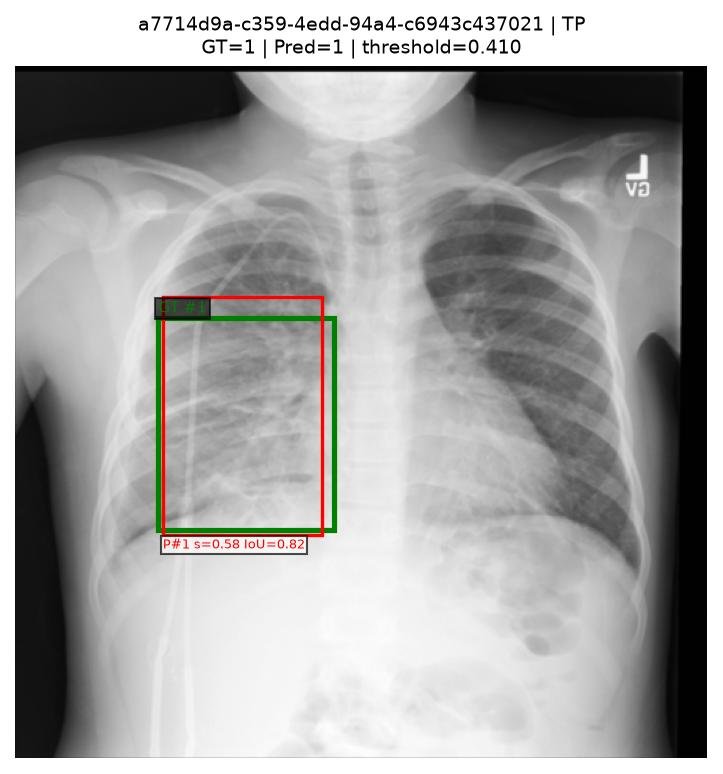
\includegraphics[width=0.45\textwidth]{Images/qualitative/r101_in_case1.jpg}%
    }
    \caption{Representative detections for case 1 produced by R50-IN and R101-IN.}
    \label{fig:representative_detections_case1}
\end{figure}

\begin{figure}[H]
    \centering
    \subfloat[R50-IN -- case 2]{%
        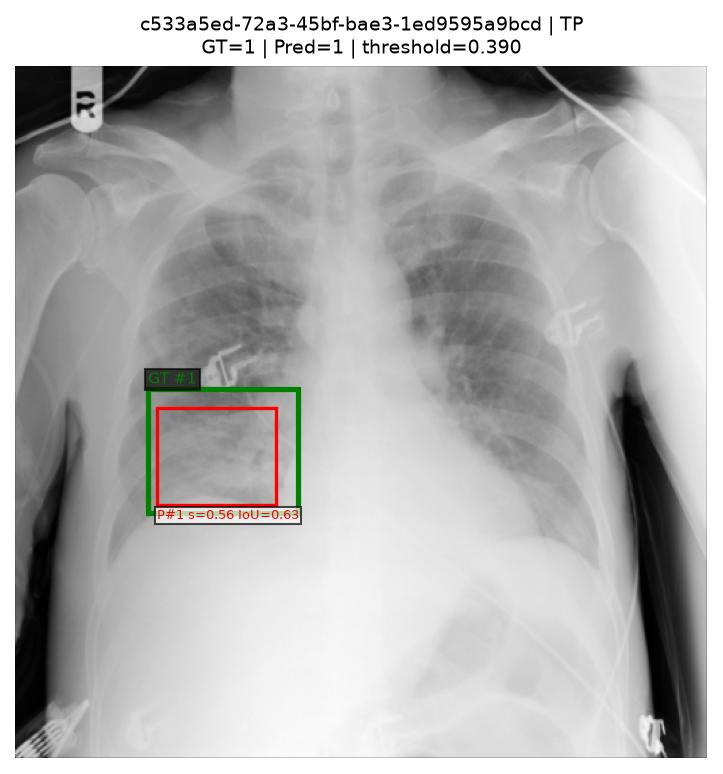
\includegraphics[width=0.45\textwidth]{Images/qualitative/r50_in_case2.jpg}%
    }
    \hfill
    \subfloat[R101-IN -- case 2]{%
        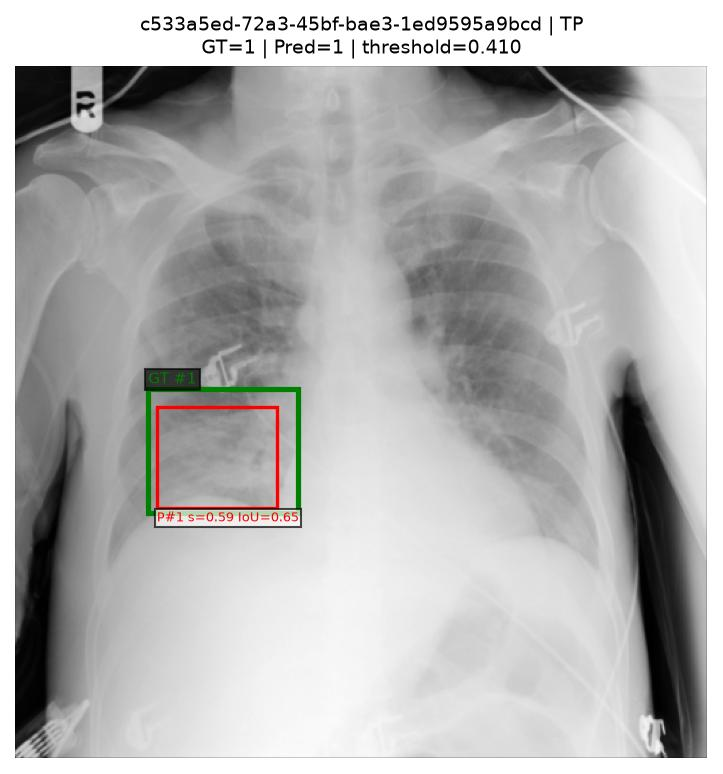
\includegraphics[width=0.45\textwidth]{Images/qualitative/r101_in_case2.jpg}%
    }
    \caption{Representative detections for case 2 produced by R50-IN and R101-IN.}
    \label{fig:representative_detections_case2}
\end{figure}

\subsection{Conclusions}
\label{subsec:conclusions_future_work}

The results show that no single configuration is best under every criterion. R50-IN achieves the highest AP ($0.423$), whereas R101-IN provides the highest $AR@10$ ($0.901$), the best image-level F1 at the Youden operating point ($0.668$), and the highest mean matched IoU ($0.692$). The deeper backbone is therefore not uniformly better, but it is competitive when recall and localization are emphasized.

The Chest-Xray-initialized models are weaker in the present experiments, especially R101-CX ($AP=0.239$). This result should not be interpreted as evidence that domain-specific pretraining is intrinsically less effective. The optimization budgets were not fully matched, and the R101 configurations required different training schedules and different amounts of fine-tuning. A controlled comparison would require comparable training budgets, repeated runs, and uncertainty estimates.

\subsection{Clinical and Dataset Limitations}
\label{subsec:clinical_limitations}

The quantitative results should also be interpreted in the context of the
information available in the dataset. A discussion with a radiologist during
the qualitative review highlighted several limitations that are difficult to
capture using detection metrics alone. In particular, the detector operates
on a single chest radiograph, whereas the clinical assessment of suspected
pneumonia can make use of additional projections and, when necessary, follow-up
examinations. Frontal and lateral views can provide complementary information
about the location and extent of an abnormality, while repeated imaging can
help distinguish persistent findings from transient ones. None of this
additional information is available to the present model.

Patient positioning is another relevant factor. Many examinations in the
RSNA dataset are portable radiographs, including images acquired from patients
who are not standing. The radiologist consulted for this study emphasized that
positioning can alter the apparent distribution and extent of pulmonary
opacities. In particular, small opacities may be less evident in supine
examinations, while more extensive areas of increased density may appear more
diffuse. The visual appearance of a lesion is therefore influenced not only by
the underlying pathology but also by acquisition conditions and patient
position.

More importantly, the radiographic pattern used by the detector is only one
part of the clinical assessment. An opacity compatible with pneumonia can also
be produced by other thoracic conditions. The consulting radiologist noted
that some neoplastic findings can have an appearance similar to infection on a
single chest radiograph. In a clinically uncertain case, the radiographic
finding may be described first as an opacity or consolidation, and its meaning
is then assessed together with symptoms, medical history and previous imaging.
If the abnormality persists despite an initial clinical treatment, additional
imaging such as CT may be required to clarify the diagnosis. This means that a
prediction that disagrees with a dataset label should not automatically be
interpreted as a clinically incorrect observation.

The same issue became evident in the inspection of individual predictions from
R101-IN. Figure~\ref{fig:clinical_examples} shows two representative cases
selected during the radiological review. In the first example, the model marks
an opacity adjacent to an enlarged cardiac silhouette. The opacity itself can
look compatible with pneumonia, but the radiologist considered the cardiac
silhouette and the overall thoracic appearance essential for interpretation.
In this case, the increased density was considered more consistent with a
cardiocirculatory condition than with pneumonia. The example illustrates that
a model focusing mainly on the local appearance of an opacity may miss
information contained in the surrounding anatomy, such as the heart size.

In the second example, R101-IN predicts pneumonia, while the consulting
radiologist considered the overall appearance more compatible with atelectasis.
The distinction was not based on the opacity alone. Other radiographic signs,
including changes involving the costophrenic angles and the diaphragm, were
considered together with the appearance and extent of the opacity. These signs
are not explicitly represented in the current prediction target, which is
primarily based on the location and size of the annotated bounding box.

\begin{figure}[H]
    \centering
    \subfloat[Opacity adjacent to an enlarged cardiac silhouette.\label{fig:clinical_case_heart}]{%
        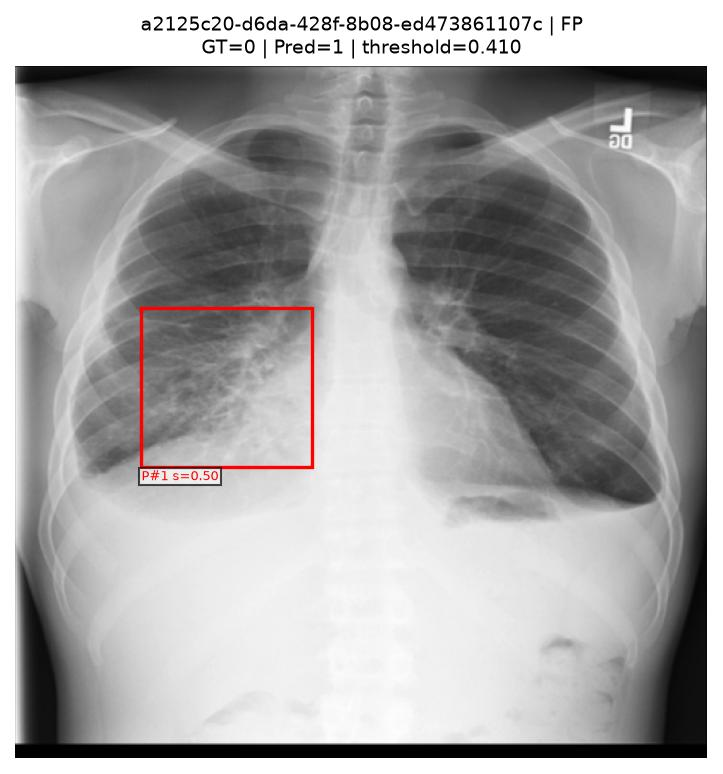
\includegraphics[width=0.4\textwidth]{Images/qualitative/clinical_case_heart.jpg}%
    }
    \hfill
    \subfloat[R101-IN prediction considered compatible with atelectasis.\label{fig:clinical_case_atelectasis}]{%
        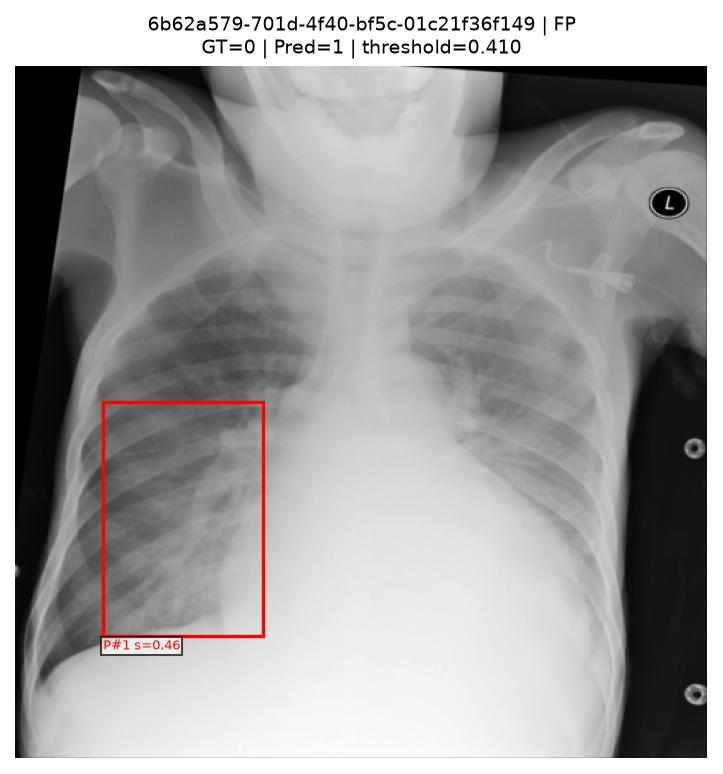
\includegraphics[width=0.4\textwidth]{Images/qualitative/clinical_case_atelectasis.jpg}%
    }
    \caption{Two R101-IN predictions discussed during the radiological review. The examples illustrate cases in which interpretation depends on the global radiographic appearance and on findings beyond the annotated opacity itself.}
    \label{fig:clinical_examples}
\end{figure}

These cases also highlight a limitation of using the confidence associated with
a single predicted box as a direct proxy for diagnostic certainty. A large or
high-confidence prediction is not necessarily more clinically plausible than a
smaller one if the surrounding radiographic findings point towards another
explanation. Conversely, an extensive pneumonia is possible, but its clinical
plausibility still depends on the complete presentation. Future systems could
therefore benefit from calibrating the interpretation of detection confidence
with the spatial extent of the predicted region and with additional anatomical
features rather than relying on the box score alone.

The discussion also raises a question about the quality of the ground truth.
The RSNA dataset is strongly imbalanced at image level, but the appropriate
response is not necessarily to give greater weight to all positive examples.
If a subset of positive or negative cases is clinically ambiguous, simple
reweighting can increase the influence of uncertain annotations without
improving the underlying supervision. A more useful strategy would be to
identify and review difficult cases, characterize potentially ambiguous
negatives, and, where possible, obtain stronger expert consensus annotations.
This would make it possible to separate limitations of the detector from
limitations of the reference labels more reliably.

At the same time, the radiological review was positive about the overall
quality of the proposed detector. In particular, the radiologist considered
false positives to be less concerning, on average, than missed findings in the
context of pneumonia screening. This observation does not imply that false
positives are clinically irrelevant, but it supports the importance of
maintaining high sensitivity when choosing an operating point. The present
results are consistent with this perspective: R101-IN does not achieve the
highest AP, but it provides the highest recall and the strongest image-level
balance at the selected operating point.

Overall, the project shows that the FCOS-style detector is able to provide a
compact anchor-free framework for pneumonia localization and that backbone
depth, initialization and optimization have a measurable effect on the
results. The clinical review, however, shows that localization from a single
radiograph is only a partial approximation of the diagnostic process. A more
complete system could combine frontal and lateral radiographs when available,
anatomical measurements such as cardiac and diaphragmatic information,
selected clinical history, and additional examinations such as CT in difficult
cases. Such a system would use the detector as a spatially grounded component
rather than treating its output as a complete diagnosis.

The main lesson is therefore not simply that a deeper or differently
initialized backbone is preferable. The results suggest that improvements in
the data and in the information presented to the model may be at least as
important as increasing model complexity. Future experiments should first make
the training comparison more controlled and the clinical characterization of
the dataset more rigorous. This would provide a stronger basis for determining
which architectural improvements genuinely improve pneumonia localization and
which apparent errors are instead related to the ambiguity of the underlying
radiographic evidence.


\section{Code and Dataset Availability}
\label{sec:code_dataset_availability}

The complete implementation of the proposed detection pipeline, including the
backbone, FPN, detection heads, training procedures, and evaluation scripts,
is available in the project repository:

\begin{center}
\url{https://github.com/Francesco2035/fcos-pneumonia-detection-naml-25-26}
\end{center}

The experiments were conducted using two publicly available chest X-ray
datasets. The main detection experiments use the RSNA Pneumonia Detection
Challenge dataset, which provides chest radiographs together with pneumonia
annotations and bounding boxes. The dataset is available through the official
RSNA challenge resources.

For backbone pretraining, the Chest-Xray initialization was obtained from the
public ``Chest X-Ray Images (Pneumonia)'' dataset, containing Normal and
Pneumonia images for binary classification.

The corresponding dataset resources are available at:

\begin{itemize}
    \item RSNA Pneumonia Detection Challenge:
    \href{https://www.rsna.org/challenge-datasets/2018}{RSNA official dataset page}
    
    \item Chest X-Ray Images (Pneumonia):
    \href{https://www.kaggle.com/datasets/paultimothymooney/chest-xray-pneumonia}{Kaggle dataset page}
\end{itemize}

\section{Acknowledgements}

The author would like to thank Dr.~Cristina Tartaglia, radiologist at
Gallipoli Hospital, for her valuable support during the qualitative analysis
of the results. Her clinical feedback was particularly helpful in interpreting
ambiguous radiographic findings and in discussing the limitations of assessing
pneumonia from single chest X-ray images.

\bibliography{bibliography}

\cleardoublepage



\end{document}
